\documentclass[12pt]{article}

\usepackage{template}

% Disable indentation on new paragraphs
\setlength{\parindent}{0pt}

% Line spacing 1.5
\renewcommand{\baselinestretch}{1.5}

% Optional: graphic path
% \graphicspath{PATH_TO_GRAPHIC_FOLDER}

% To use Times font family, uncomment this row
% \usepackage{mathptmx}

% To use roman section / subsection, uncomment these rows
% \renewcommand{\thesection}{\Roman{section}}
% \renewcommand{\thesubsection}{\thesection.\Roman{subsection}}

% Define course name, report name and report title.
\newcommand{\coursename}{Thực hành Cấu trúc dữ liệu và giải thuật}
\newcommand{\reportname}{CÁC THUẬT TOÁN SẮP XẾP}
\newcommand{\reporttitle}{BÁO CÁO ĐỒ ÁN}

\newcommand{\studentname}{
    Lê Hải Sơn - 23120162 \\[-0.1cm]
    Lê Đức Thành - 23120165 \\[-0.1cm]
    Đặng Ngọc Tiên - 23120171 \\[-0.1cm]
    Khổng Đức Tiến - 23120175 \\[-0.1cm]
    Nguyễn Hồ Anh Tuấn - 23120185}

\newcommand{\teachername}{Thầy Trần Hoàng Quân}

% Header
\lhead{Các thuật toán sắp xếp}
\rhead{Thực hành Cấu trúc dữ liệu và giải thuật}

% ============ DOCUMENT ============
\begin{document}

\begin{titlepage}
\newcommand{\HRule}{\rule{\linewidth}{0.5mm}}
\centering

\vspace*{-2cm}
\textsc{\Large TRƯỜNG ĐẠI HỌC KHOA HỌC TỰ NHIÊN, ĐHQG-HCM}\\[0.3cm]
\textsc{\Large KHOA CÔNG NGHỆ THÔNG TIN}\\[1cm]


\includegraphics[scale=.40]{img/logo_hcmus.png}\\

\HRule \\[0.3cm]
{ 
\Large{\bfseries{\reporttitle}}\\
\Large\bfseries Đề tài: \huge{\bfseries{\reportname}}\\[0.5cm]
\Large{\bfseries{Môn học: \coursename}}
}\\[0.3cm]
\HRule \\[0.3cm]

\begin{minipage}[t]{0.45\textwidth}
\begin{flushleft} \large
\emph{Nhóm sinh viên thực hiện:}\\
\studentname
\end{flushleft}
\end{minipage}
~
\begin{minipage}[t]{0.4\textwidth}
\begin{flushright} \large
\emph{Giáo viên hướng dẫn:} \\
\teachername
\end{flushright}
\end{minipage}\\[3.5cm]

\Large Thành phố Hồ Chí Minh, tháng 1 năm 2025

\vfill
\end{titlepage}

\pagenumbering{arabic}
\setcounter{tocdepth}{2}
\setcounter{page}{2}

\tableofcontents
\pagebreak

\section{Thông tin về nhóm}

Trang này chứa các thông tin về nhóm.
\pagebreak

\section{Giới thiệu}

Đồ án này được thực hiện trong khuôn khổ môn học \textit{Cấu trúc dữ liệu 
và giải thuật} tại Khoa Công nghệ thông tin, Trường Đại học Khoa học tự nhiên, 
ĐHQG-HCM. Đây là một môn học cốt lõi, giúp sinh viên nắm vững các 
khái niệm cơ bản về giải thuật, phân tích độ phức tạp và ứng dụng 
thực tế trong lập trình. Thông qua đồ án này, sinh viên sẽ có cơ hội 
thực hành sâu hơn về \textit{các thuật toán sắp xếp} – một trong những chủ đề 
quan trọng nhất trong lĩnh vực giải thuật. Mục tiêu chính là giúp 
sinh viên hiểu rõ cách các thuật toán sắp xếp hoạt động, các trường hợp 
ứng dụng cụ thể, cũng như cách đánh giá hiệu quả của từng thuật toán 
dựa trên các tiêu chí như \textit{thời gian thực thi} và \textit{số phép so sánh}.
\\\\
Đồ án tập trung vào việc khảo sát và phân tích \textit{các thuật toán sắp 
xếp}, từ các thuật toán cơ bản như \textbf{Selection Sort}, \textbf{Bubble 
Sort}, \textbf{Shaker Sort}, cũng như thuật toán \textbf{Insertion Sort} 
và thuật toán biến thể của nó là \textbf{Shell Sort}, đến các thuật toán 
nâng cao như \textbf{Merge Sort}, \textbf{Quick Sort} và \textbf{Heap 
Sort}. Ngoài ra, một số thuật toán ít phổ biến và nâng cao hơn như 
\textbf{Counting Sort}, \textbf{Radix Sort} và \textbf{Flash Sort} cũng 
được đưa vào nghiên cứu để mở rộng kiến thức của sinh viên. Để đảm bảo 
tính toàn diện, đồ án yêu cầu thực hiện các bước: lý thuyết thuật toán, 
cài đặt thuật toán, thực nghiệm trên các loại dữ liệu đầu vào khác nhau, 
đo lường hiệu suất và phân tích kết quả thông qua các bảng biểu và biểu 
đồ, rồi đưa ra nhận xét riêng cho từng kiểu dữ liệu, kích thước đầu vào 
với các thuật toán tương ứng. Đồng thời, đồ án cũng đưa ra các nhận xét 
tổng thể mang tính thiết thực, tóm gọn lại những gì đã nêu trên.
\\\\
Phần lý thuyết cung cấp nền tảng cơ bản về ý tưởng, cách hoạt động và độ 
phức tạp của các thuật toán được chọn cùng đưa ra các ví dụ đi kèm. Phần 
cài đặt thuật toán trình bày mã nguồn C++ và giải thích chi tiết cách 
triển khai từng thuật toán. Phần thực nghiệm và phân tích bao gồm các 
kết quả đo lường (về thời gian chạy, số phép so sánh) rồi so sánh hiệu 
suất của các thuật toán trong các trường hợp đầu vào khác nhau. Cuối cùng, 
phần kết luận đưa ra nhận xét tổng quan về hiệu quả của các thuật toán, 
các trường hợp sử dụng tối ưu và bài học rút ra từ đồ án. Đây là một bước 
đệm quan trọng giúp sinh viên phát triển tư duy thuật toán cũng như kỹ 
năng lập trình, chuẩn bị cho các môn học nâng cao và các dự án thực tế 
trong tương lai. Đồ án này không chỉ giúp sinh viên nắm vững kiến thức 
chuyên môn mà còn rèn luyện khả năng làm việc nhóm, giải quyết vấn đề và 
trình bày kết quả một cách chuyên nghiệp. 
\pagebreak

\section{Các thuật toán sắp xếp}

\subsection{Insertion Sort}

%Là thuật toán sắp xếp dựa trên phương pháp chèn trực tiếp. Thuật toán hoạt động hiệu quả trên mảng nhỏ hoặc mảng gần như đã sắp xếp.

\subsubsection{Ý tưởng}

Thuật toán này chia mảng thành hai phần: phần đã sắp xếp và 
phần chưa sắp xếp. Với mỗi phần tử trong mảng chưa sắp xếp, thuật toán chèn nó vào vị trí thích hợp trong phần đã sắp xếp.

\subsubsection{Mã giả}

\begin{algorithm}[H]
\caption{Insertion Sort}
\SetKwFunction{InsertionSort}{InsertionSort}
\SetKwProg{Fn}{Function}{:}{}
\Fn{\InsertionSort{a\KwSty{[]}, n}}{
    \For{$i \gets 1$ \KwTo $n$}{
        $key \gets a[i]$ \\
        $j \gets i - 1$ \\
        \While{$j \geq 0$ \KwSty{and} $a[j] > key$}{
            // Di chuyển phần tử lớn hơn sang phải \\
            $a[j + 1] \gets a[j]$ \\
            $j \gets j - 1$ \\
        }
        // Chèn key vào đúng vị trí \\
        $a[j + 1] \gets key$
    }
}
\textbf{end function}
\end{algorithm}

\subsubsection{Ví dụ}

\begin{tikzpicture}[node distance=0cm, font=\sffamily, every node/.style={minimum width=1cm, minimum height=1cm, outer sep=0pt, anchor = west}, line join=miter, line cap=rect]
	
	% Trạng thái ban đầu
	\node[font=\rmfamily] at (0, 0) {Giả sử ta có mảng ban đầu với $n=6$ như sau:};
	\node[draw, fill=white] at (9, 0) {6};
	\node[draw, fill=white] at (10, 0) {1};
	\node[draw, fill=white] at (11, 0) {4};
	\node[draw, fill=white] at (12, 0) {8};
	\node[draw, fill=white] at (13, 0) {2};
	\node[draw, fill=white] at (14, 0) {15};
	
	% Trạng thái 1
	\node[font=\rmfamily] at (0, -1) {{\bfseries Bước 1:} Bắt đầu từ vị trí $i=1$, chèn 1 vào đúng vị trí của phần mảng đã sắp xếp (chỉ có 6).};
	\node[draw, fill=white] at (1, -2.5) {6};
	\node[draw, fill=yellow] at (2, -2.5) {1};
	\node[draw, fill=white] at (3, -2.5) {4};
	\node[draw, fill=white] at (4, -2.5) {8};
	\node[draw, fill=white] at (5, -2.5) {2};
	\node[draw, fill=white] at (6, -2.5) {15};
	\draw[line width=0.7mm, shorten <=0pt] (2.5, -2) -- (2.5, -1.5);
	\draw[line width=0.7mm] (2.5, -1.5) -- (1, -1.5);
	\draw[->, line width=0.7mm, shorten >=0pt] (1, -1.5) -- (1,-2);
	
	\draw[->, line width=0.7mm] (8, -2.5) -- (9.5, -2.5);
	
	\node[draw, fill=blue] at (10.5, -2.5) {1};
	\node[draw, fill=blue] at (11.5, -2.5) {6};
	\node[draw, fill=white] at (12.5, -2.5) {4};
	\node[draw, fill=white] at (13.5, -2.5) {8};
	\node[draw, fill=white] at (14.5, -2.5) {2};
	\node[draw, fill=white] at (15.5, -2.5) {15};
	
	% Trạng thái 2
	\node[font=\rmfamily] at (0, -4) {{\bfseries Bước 2:} Với vị trí $i=2$, chèn 4 vào đúng vị trí của phần mảng đã sắp xếp (gồm 1, 6).};
	\node[draw, fill=white] at (1, -5.5) {1};
	\node[draw, fill=white] at (2, -5.5) {6};
	\node[draw, fill=yellow] at (3, -5.5) {4};
	\node[draw, fill=white] at (4, -5.5) {8};
	\node[draw, fill=white] at (5, -5.5) {2};
	\node[draw, fill=white] at (6, -5.5) {15};
	\draw[line width=0.7mm, shorten <=0pt] (3.5, -5) -- (3.5, -4.5);
	\draw[line width=0.7mm] (3.5, -4.5) -- (2, -4.5);
	\draw[->, line width=0.7mm, shorten >=0pt] (2, -4.5) -- (2,-5);
	
	\draw[->, line width=0.7mm] (8, -5.5) -- (9.5, -5.5);
	
	\node[draw, fill=blue] at (10.5, -5.5) {1};
	\node[draw, fill=blue] at (11.5, -5.5) {4};
	\node[draw, fill=blue] at (12.5, -5.5) {6};
	\node[draw, fill=white] at (13.5, -5.5) {8};
	\node[draw, fill=white] at (14.5, -5.5) {2};
	\node[draw, fill=white] at (15.5, -5.5) {15};
		
\end{tikzpicture}

\pagebreak

\begin{tikzpicture}[node distance=0cm, font=\sffamily, every node/.style={minimum width=1cm, minimum height=1cm, outer sep=0pt, anchor = west}, line join=miter, line cap=rect]
	
	% Trạng thái 3
	\node[font=\rmfamily, text width=18cm] at (0, 0) {{\bfseries Bước 3:} Với $i=3$, không thay đổi vị trí của 8 vì nó lớn hơn tất cả phần tử trong phần mảng \par đã sắp xếp.};
	\node[draw, fill=white] at (1, -1.5) {1};
	\node[draw, fill=white] at (2, -1.5) {4};
	\node[draw, fill=white] at (3, -1.5) {6};
	\node[draw, fill=yellow] at (4, -1.5) {8};
	\node[draw, fill=white] at (5, -1.5) {2};
	\node[draw, fill=white] at (6, -1.5) {15};
	\draw[line width=0.7mm, shorten <=0pt] (4.5, -1) -- (4.5, -0.5);
	\draw[line width=0.7mm] (4.5, -0.5) -- (4, -0.5);
	\draw[->, line width=0.7mm, shorten >=0pt] (4, -0.5) -- (4, -1);
	
	\draw[->, line width=0.7mm] (8, -1.5) -- (9.5, -1.5);
	
	\node[draw, fill=blue] at (10.5, -1.5) {1};
	\node[draw, fill=blue] at (11.5, -1.5) {4};
	\node[draw, fill=blue] at (12.5, -1.5) {6};
	\node[draw, fill=blue] at (13.5, -1.5) {8};
	\node[draw, fill=white] at (14.5, -1.5) {2};
	\node[draw, fill=white] at (15.5, -1.5) {15};
	
	% Trạng thái 4
	\node[font=\rmfamily, text width=20cm] at (0, -3) {{\bfseries Bước 4:} Tương tự, với $i=4$, chèn 2 vào đúng vị trí.};
	\node[draw, fill=white] at (1, -4.5) {1};
	\node[draw, fill=white] at (2, -4.5) {4};
	\node[draw, fill=white] at (3, -4.5) {6};
	\node[draw, fill=white] at (4, -4.5) {8};
	\node[draw, fill=yellow] at (5, -4.5) {2};
	\node[draw, fill=white] at (6, -4.5) {15};
	\draw[line width=0.7mm, shorten <=0pt] (5.5, -4) -- (5.5, -3.5);
	\draw[line width=0.7mm] (5.5, -3.5) -- (2, -3.5);
	\draw[->, line width=0.7mm, shorten >=0pt] (2, -3.5) -- (2, -4);
	
	\draw[->, line width=0.7mm] (8, -4.5) -- (9.5, -4.5);
	
	\node[draw, fill=blue] at (10.5, -4.5) {1};
	\node[draw, fill=blue] at (11.5, -4.5) {2};
	\node[draw, fill=blue] at (12.5, -4.5) {4};
	\node[draw, fill=blue] at (13.5, -4.5) {6};
	\node[draw, fill=blue] at (14.5, -4.5) {8};
	\node[draw, fill=white] at (15.5, -4.5) {15};
	
	% Trạng thái 5
	\node[font=\rmfamily, text width=20cm] at (0, -6) {{\bfseries Bước 5:} Cuối cùng, sau khi chèn 15 vào đúng vị trí, ta thu được mảng đã sắp xếp.};
	\node[draw, fill=white] at (1, -7.5) {1};
	\node[draw, fill=white] at (2, -7.5) {4};
	\node[draw, fill=white] at (3, -7.5) {6};
	\node[draw, fill=white] at (4, -7.5) {8};
	\node[draw, fill=white] at (5, -7.5) {2};
	\node[draw, fill=yellow] at (6, -7.5) {15};
	\draw[line width=0.7mm, shorten <=0pt] (6.5, -7) -- (6.5, -6.5);
	\draw[line width=0.7mm] (6.5, -6.5) -- (6, -6.5);
	\draw[->, line width=0.7mm, shorten >=0pt] (6, -6.5) -- (6, -7);
	
	\draw[->, line width=0.7mm] (8, -7.5) -- (9.5, -7.5);
	
	\node[draw, fill=blue] at (10.5, -7.5) {1};
	\node[draw, fill=blue] at (11.5, -7.5) {2};
	\node[draw, fill=blue] at (12.5, -7.5) {4};
	\node[draw, fill=blue] at (13.5, -7.5) {6};
	\node[draw, fill=blue] at (14.5, -7.5) {8};
	\node[draw, fill=blue] at (15.5, -7.5) {15};
	
\end{tikzpicture}

\subsubsection{Độ phức tạp thuật toán}

\begin{itemize}
    \item Độ phức tạp thời gian
    \begin{itemize}[label=$\circ$]
        \item Trường hợp tốt nhất: $O(n)$ khi mảng đã được sắp xếp.
        \item Trường hợp xấu nhất: $O\left(n^2\right)$ khi mảng sắp xếp 
        ngược, cần dịch chuyển toàn bộ phần tử cho mỗi lần chèn.
        \item Trường hợp trung bình: $O\left(n^2\right)$ do phải thực 
        hiện n lần chèn và mỗi lần chèn có thể phải dịch chuyển trung 
        bình n/2 phần tử.
    \end{itemize}
    \item Độ phức tạp không gian: $O\left(1\right)$ vì là thuật toán 
    sắp xếp tại chỗ (in-place), không sử dụng bộ nhớ phụ ngoài biến tạm.
\end{itemize}

\subsubsection{Các cải tiến của thuật toán}

\begin{enumerate}
    \item Binary Insertion Sort
    \begin{itemize}
        \item Ý tưởng: Thay vì sử dụng tìm kiếm tuyến tính để tìm vị trí 
        chèn phù hợp trong mảng đã sắp xếp thì ta có thể sử dụng thuật 
        toán làm việc được trên mảng đã sắp xếp để có thể tối ưu việc 
        tìm vị trí phù hợp để chèn. Đó chính là Binary Search để có 
        thể tìm kiếm tốt hơn với độ phức tạp của thuật toán là 
        $O\left(\log{n}\right)$.
        \item Ví dụ: Trong mảng $A=\left[1,4,5,10,15,20,9,21\right]$. 
        Khi xét vị trí $i=7$, ta cần tìm vị trí phụ hợp để chèn 9 
        vào thì có thể dùng binary search trong mảng đã sắp xếp trước 
        đó $\left[1,4,5,10,15,20\right]$ để tìm vị trí thích hợp.
    \end{itemize}
    \item Library Sort (còn gọi là gapped insertion sort)
    \begin{itemize}
        \item Ý tưởng: Thuật toán này có thể sử dụng các khoảng trống 
        (gaps) trong mảng để chèn phần tử, giúp hạn chế việc dịch 
        chuyển quá nhiều khi chèn giúp tối ưu trong việc xử lí khi 
        mảng có rất nhiều phần tử. Khi khoảng trống hết, mảng sẽ được 
        mở rộng và phân bổ lại khoảng trống mới. Với độ phức tạp thời 
        gian trung bình của Library Sort là $O\left(n\log{n}\right)$.
        \item Ví dụ: Với mảng $A=\left[3,4,5,8,1,2\right]$. Sau khi 
        tạo mảng với khoảng trống và chèn 3, 4, 5, 8 thì mảng 
        như sau $\left[3,\_,4,5,8\right]$.
        \begin{itemize}[label=$\circ$]
            \item Như vậy, khi chèn 1 vào đúng vị trí thì sẽ sắp xếp 
            lại và điền vào khoảng trống $\left[1,3,4,5,8\right]$.
            \item Tiếp theo, chèn 2, mảng không còn vị trí nào sau 
            phần tử 3 thì khi chèn 2 thì lúc này khoảng trống sẽ hết 
            thì mảng sẽ được mở rộng và phân bổ lại khoảng trống mới. 
            Mảng lúc này sẽ là $\left[1,\_,\_,3,4,5,8\right]$ khi đó 
            khi chèn 2 vào thì sẽ sử dụng khoảng trống mới mở rộng 
            $\left[1,2,\_,3,4,5,8\right]$.
        \end{itemize}
    \end{itemize}
\end{enumerate}
\subsection{Selection Sort}

Là một thuật toán sắp xếp đơn giản dựa trên việc tìm kiếm 
và đặt phần tử nhỏ nhất (hoặc lớn nhất) vào đúng vị trí 
của nó trong danh sách. Thuật toán này được gọi là "Selection" 
vì mỗi lần lặp, nó chọn phần tử phù hợp để đặt vào vị trí 
chính xác. Đây là một thuật toán không ổn định (unstable) 
vì nếu các phần tử có giá trị bằng nhau, thứ tự ban đầu có thể 
bị thay đổi do hoán vị.

\subsubsection{Ý tưởng}

\begin{enumerate}
    \item Chia danh sách thành hai phần:
    \begin{itemize}[label=$\circ$]
        \item Phần đã sắp xếp (ban đầu trống).
        \item Phần chưa sắp xếp (ban đầu chứa toàn bộ danh sách).
    \end{itemize}
    \item Lặp qua danh sách:
    \begin{itemize}[label=$\circ$]
        \item Tìm phần tử nhỏ nhất trong phần chưa sắp xếp.
        \item Hoán đổi phần tử nhỏ nhất này với phần tử đầu tiên 
        của phần chưa sắp xếp.
    \end{itemize}
    \item Sau mỗi lần hoán đổi, mở rộng phần đã sắp xếp thêm 
    một phần tử.
    \item Tiếp tục cho đến khi toàn bộ danh sách được sắp xếp.
\end{enumerate}

\subsubsection{Mã giả}

\begin{algorithm}[H]
\caption{Selection Sort}
\SetKwFunction{SelectionSort}{SelectionSort}
\SetKwProg{Fn}{Function}{:}{}
\Fn{\SelectionSort{a\KwSty{[]}, n}}{
    \For{$i \gets 0$ \KwTo $n-2$}{
        // Bước 1: Giả định phần tử nhỏ nhất là a[i] \\
        $minIndex \gets i$ \\
        // Bước 2: Tìm phần tử nhỏ nhất trong phần chưa sắp xếp \\
        \For{$j \gets i+1$ \KwTo $n-1$}{
            \If{$a[j] < a[minIndex]$}{
                $minIndex \gets j$ \\
            }
        }
        // Bước 3: Hoán đổi phần tử nhỏ nhất với a[i] \\
        \If{$minIndex \neq i$}{
            swap($a[i]$, $a[minIndex]$) \\
        }
    }
}
\textbf{end function}
\end{algorithm}

\subsubsection{Ví dụ}

\subsubsection{Độ phức tạp thuật toán}

\begin{itemize}
    \item Độ phức tạp thời gian
    \begin{itemize}[label=$\circ$]
        \item Trường hợp tốt nhất: $O\left(n^2\right)$.
        \item Trường hợp xấu nhất: $O\left(n^2\right)$.
        \item Trung bình: $O\left(n^2\right)$ vì thuật toán sử dụng 
        hai vòng lặp lồng nhau để tìm phần tử nhỏ nhất.
    \end{itemize}
    \item Độ phức tạp không gian: $O\left(1\right)$ vì không sử dụng 
    bộ nhớ bổ sung ngoài danh sách ban đầu.
\end{itemize}
\subsection{Shell Sort}

Là một thuật toán sắp xếp dựa trên sắp xếp chèn (Insertion Sort), được 
đặt theo tên của người phát minh, Donald Shell. Thuật toán này cải tiến 
sắp xếp chèn bằng cách cho phép so sánh và hoán đổi các phần tử cách xa 
nhau trước khi thu hẹp khoảng cách lại. Điều này giúp giảm thiểu số lần 
hoán đổi và dịch chuyển các phần tử. Đây là một thuật toán không ổn định, 
phần tử bằng nhau có thể bị đổi chỗ do hoán đổi các nhóm cách xa nhau.

\subsubsection{Ý tưởng}

\begin{enumerate}
    \item Thay vì sắp xếp toàn bộ danh sách một cách tuần tự, Shell Sort 
    chia danh sách thành các danh sách con với khoảng cách giữa các phần 
    tử được xác định bởi một giá trị gọi là khoảng cách (interval).
    \item Thuật toán sử dụng sắp xếp chèn để sắp xếp các phần tử trong 
    từng danh sách con này.
    \item Sau mỗi vòng lặp, khoảng cách được thu nhỏ dần, cuối cùng trở 
    về 1, lúc này danh sách được sắp xếp hoàn chỉnh.
\end{enumerate}

\subsubsection{Mã giả}

\begin{algorithm}[H]
\caption{Shell Sort}
\SetKwFunction{ShellSort}{ShellSort}
\SetKwProg{Fn}{Function}{:}{}
\Fn{\ShellSort{a\KwSty{[]}, n}}{
    // Bước 1: Khởi tạo khoảng cách \\
    $gap \gets n / 2$ \\
    \While{$gap > 0$}{
        // Bước 2: Sắp xếp chèn với khoảng cách gap \\
        \For{$i \gets gap$ \KwTo $n - 1$}{
            $temp \gets a[i]$ \\
            $j \gets i$ \\
            // Dịch chuyển các phần tử lớn hơn temp lên một khoảng cách \\
            \While{$j \geq gap$ \KwSty{and} $a[j - gap] > temp$}{
                $a[j] \gets a[j - gap]$ \\
                $j \gets j - gap$ \\
            }
            // Đặt temp vào đúng vị trí \\
            $a[j] \gets temp$ \\
        }
        // Bước 3: Giảm khoảng cách \\
        $gap \gets gap / 2$ \\
    }
}
\textbf{end function}
\end{algorithm}

\subsubsection{Ví dụ}

\subsubsection{Độ phức tạp thuật toán}

\begin{itemize}
    \item Độ phức tạp thời gian
    \begin{itemize}[label=$\circ$]
        \item Trường hợp tốt nhất: $O\left(n\log{n}\right)$, khi dữ liệu gần như đã được sắp xếp.
        \item Trường hợp xấu nhất: $O\left(n^2\right)$.
        \item Trường hợp trung bình: $O\left(n^{3/2}\right)$.
    \end{itemize}
    \item Độ phức tạp không gian: $O\left(1\right)$.
\end{itemize}
\subsection{Bubble Sort}

\subsubsection{Ý tưởng}

Trong thuật toán này, dãy các phần tử sẽ được duyệt từ đầu mảng đến 
cuối mảng, nếu hai phần tử kề nhau bị sai thứ tự thì đổi chỗ của chúng 
cho nhau. Sau lượt duyệt như vậy, phần tử lớn nhất sẽ được chuyển về 
vị trí cuối mảng giống như tên gọi - “nổi bọt”. Sau đó ta tiếp tục 
duyệt từ đầu mảng đến vị trí kế cuối mảng,... cứ như vậy cho đến khi 
mảng được sắp xếp.

\subsubsection{Mã giả}

\begin{algorithm}[H]
\caption{Bubble Sort}
\SetKwFunction{BubbleSort}{BubbleSort}
\SetKwProg{Fn}{Function}{:}{}
\Fn{\BubbleSort{a\KwSty{[]}, n}}{
    \For{$i \gets 0$ \KwTo $n - 2$}{
        \For{$j \gets 0$ \KwTo $n - i - 2$}{
            // Nếu sai vị trí thì hoán vị \\
            \If{$a[j] > a[j + 1]$}{
                swap($a[j]$, $a[j + 1]$)
            }
        }
    }
}
\textbf{end function}
\end{algorithm}

\subsubsection{Ví dụ}

\subsubsection{Độ phức tạp thuật toán}

\begin{itemize}
    \item Độ phức tạp thời gian
    
    Trong thuật toán này, có $n-1$ lần lặp đối với biến $i$, mỗi lần 
    sẽ đưa phần tử lớn nhất trong đoạn $a\left[0..n-i-1\right]$ về 
    vị trí $n-i-1$. Với lần lặp thứ $i$, ta thực hiện $n-i$ 
    thao tác so sánh. Do đó, tổng số phép so sánh thực hiện là:
    
    \begin{equation}
        \left(n-1\right)+\left(n-2\right)+\ldots+2+1
        =\frac{n\left(n-1\right)}{2}\approx n^2
    \end{equation}
        
    Có thể thấy thuật toán không phụ thuộc vào phân bố ban đầu của dữ 
    liệu, ta có:
    
    \begin{itemize}[label=$\circ$]
        \item Trường hợp tốt nhất: $O\left(n^2\right)$.
        \item Trường hợp xấu nhất: $O\left(n^2\right)$.
        \item Trường hợp trung bình: $O\left(n^2\right)$.
    \end{itemize}
    
    \item Độ phức tạp không gian: $O\left(1\right)$.
\end{itemize}
\subsection{Heap Sort}

\subsubsection{Ý tưởng}

\begin{itemize}
    \item Xây dựng Max-Heap: Chuyển đổi mảng đầu vào thành một Max-Heap, 
    sao cho phần tử lớn nhất nằm ở gốc cây.
    \item Sắp xếp:
    \begin{enumerate}
        \item Hoán đổi phần tử gốc (lớn nhất) với phần tử cuối cùng 
        của mảng.
        \item Giảm kích thước của heap đi 1 và gọi hàm Heapify để 
        duy trì tính chất Max-Heap.
        \item Lặp lại quá trình này cho đến khi heap chỉ còn một phần tử.
    \end{enumerate}
\end{itemize}

\subsubsection{Mã giả}

\begin{algorithm}[H]
\caption{Heap Sort}
\SetKwFunction{Heapify}{heapify}
\SetKwFunction{HeapSort}{HeapSort}
\SetKwProg{Fn}{Function}{:}{}
\Fn{\Heapify{a\KwSty{[]}, n, i}}{
    $largest \gets i$ \\
    $left \gets 2 * i + 1$ \\
    $right \gets 2 * i + 2$ \\
    \If{$left < n$ \KwSty{and} $a[left] > a[largest]$}{
        $largest \gets left$ \\
    }
    \If{$right < n$ \KwSty{and} $a[right] > a[largest]$}{
        $largest \gets right$ \\
    }
    \If{$largest \neq i$}{
        // Đổi chỗ root với phần tử lớn nhất \\
        swap($a[i]$, $a[largest]$) \\
        // Đệ quy heapify trên node bị ảnh hưởng \\
        \Heapify{a, n, largest} \\
    }
}
\textbf{end function}

\Fn{\HeapSort{a\KwSty{[]}, n}}{
    // Bước 1: Xây dựng Max-Heap từ node trong cuối cùng \\
    \For{$i \gets \lfloor n / 2 \rfloor - 1$ \KwSty{downto} $0$}{
        \Heapify{a, n, i} \\
    }
    // Bước 2: Sắp xếp mảng bằng cách trích xuất các phần tử lớn nhất \\
    \For{$i \gets n - 1$ \KwSty{downto} $1$}{
        swap($a[0]$, $a[i]$) \\
        \Heapify{a, i, 0} \\
    }
}
\textbf{end function}
\end{algorithm}

\subsubsection{Ví dụ}

\subsubsection{Độ phức tạp thuật toán}

\begin{itemize}
    \item Độ phức tạp thời gian
    \begin{itemize}[label=$\circ$]
        \item Trường hợp tốt nhất: $O(n\log{n})$ vì khi xây dựng heap 
        và thực hiện thao tác heapify vẫn cần $O(n \log n)$ do tính 
        chất của heap.
        \item Trường hợp xấu nhất: $O(n\log{n})$ trong trường hợp tệ 
        nhất (mảng hoàn toàn ngược hoặc có cấu trúc phức tạp) vẫn duy 
        trì $O(n \log n)$ vì mọi thao tác chính đều dựa trên việc 
        heapify từng phần tử.
        \item Trường hợp trung bình: $O(n\log{n})$ trường hợp trung bình 
        vẫn cần xây dựng heap và thực hiện n-1 lần thao tác Heapify.
    \end{itemize}
    \item Độ phức tạp không gian: $O(1)$ vì Heap Sort là thuật toán 
    sắp xếp tại chỗ (in-place), không sử dụng bộ nhớ phụ ngoài biến tạm.
\end{itemize}
\subsection{Merge Sort}

\subsubsection{Ý tưởng}

Thuật toán sắp xếp trộn sử dụng phương pháp chia để trị (divide-and-conquer). Đầu tiên, chia mảng $a[1..n]$ thành 2 mảng con có kích thước $n/2$ là $a[1..mid]$ và $a[mid + 1..n]$, sắp xếp và trộn hai mảng này lại, ta thu được mảng $n/2$ phần tử đã được sắp xếp. Để sắp xếp mảng $n/2$ phần tử ta lại tiếp tục chia thành hai mảng có $n/4$ phần tử, cứ như vậy gọi đệ quy cho đến khi mảng chỉ có 1 phần tử thì xem như là đã được sắp xếp.

\subsubsection{Mã giả}

\begin{algorithm}[H]
\caption{Merge Sort}
\label{merge-sort}

\SetKwFunction{mergeTwoArrays}{mergeTwoArrays}
\SetKwProg{Fn}{Function}{:}{}
\Fn{\mergeTwoArrays {arr\KwSty{[ ]}, arr1\KwSty{[ ]}, n1, arr2\KwSty{[ ]}, n2}}{
    $i \gets 0, \hspace{0.2cm} j \gets 0$ \\
    \While{$i < n1$ \KwSty{and} $j < n2$}{
        \If{$arr1[i] < arr2[j]$}{ 
            Thêm $arr1[i]$ vào $arr$ \\
            $++i$ \\
        }
        \Else{
            Thêm $arr2[j]$ vào $arr$ \\
            $++j$ \\
        }
    }
    \While{$i < n1$}{
        Thêm $arr1[i]$ vào $arr$ \\
        $++i$ \\
    }
    \While{$j < n2$}{
        Thêm $arr2[j]$ vào $arr$ \\
        $++j$ \\
    }
}
\textbf{end function}

\SetKwFunction{MergeSort}{MergeSort}
\SetKwProg{Fn}{Function}{:}{}
\Fn{\MergeSort {arr\KwSty{[ ]}, left, right}}{
    \If{$left < right$}{ 
        Tạo mảng $a1 = arr[left..mid]$ có $n1$ phần tử \\
        Tạo mảng $a2 = arr[mid+1..right]$ có $n2$ phần tử \\
        \MergeSort{arr, left, mid} \\
        \MergeSort{arr, mid + 1, right} \\
        \mergeTwoArrays{arr, a1, n1, a2, n2}
    }
}
\textbf{end function}
\end{algorithm}

\subsubsection{Ví dụ}

\subsubsection{Độ phức tạp thuật toán}

\begin{itemize}
    \item Độ phức tạp thời gian \\
    Mảng ban đầu có $n$ phần tử cần sắp xếp sẽ được chia đôi nhiều lần cho đến khi nó chỉ còn 1 phần tử, như vậy sẽ có $log_2{n}$ mức đệ quy. Ở mỗi mức đệ quy, ta duyệt qua các phần tử ở tất cả mảng con để thực hiện trộn nên độ phức tạp là $O(n)$. Như vậy độ phức tạp của thuật toán Merge Sort là $O(nlogn)$. Có thể thấy thuật toán không phụ thuộc vào phân bố ban đầu của dữ liệu, do đó ta có:
    \begin{itemize}[label=$\circ$]
        \item Trường hợp tốt nhất: $O(nlogn)$
        \item Trường hợp xấu nhất: $O(nlogn)$
        \item Trường hợp trung bình: $O(nlogn)$ 
    \end{itemize}
    
    \item Độ phức tạp không gian: $O(n)$, vì thuật toán cần tạo thêm không gian để chứa những phần tử từ 2 mảng con rồi mới trộn vào mảng ban đầu.
\end{itemize}
\subsection{Quick Sort}

\subsubsection{Ý tưởng}

Để sắp xếp một đoạn trong mảng, nếu đoạn đó có ít hơn 2 phần tử thì không cần phải làm gì cả. Ngược lại, nếu đoạn đó có từ 2 phần tử trở lên, ta chọn một phần tử ở chính giữa làm “chốt” (pivot), sau đó phân hoạch thành 2 đoạn nhỏ hơn sao cho các phần tử ở đoạn bên trái không lớn hơn pivot và các phần tử ở đoạn bên phải không nhỏ hơn pivot. Tiếp theo, ta áp dụng phương pháp tương tự cho 2 mảng con đó bằng cách gọi đệ quy đến từng mảng.

\subsubsection{Mã giả}

\begin{algorithm}[H]
\caption{Quick Sort}
\label{quick-sort}

\SetKwFunction{QuickSort}{QuickSort}
\SetKwProg{Fn}{Function}{:}{}
\Fn{\QuickSort {arr\KwSty{[ ]}, left, right}}{
    $i \gets left, \hspace{0.2cm} j \gets right$ \\
    $pivot = arr[left + (right - left) / 2]$ \\
    // Phân hoạch thành 2 đoạn \\
    \While{$i \leq j$}{ 
        \While{$arr[i] < pivot$}{
            $++i$ \\
        }
        \While{$arr[j] > pivot$}{
            $--j$ \\
        }
        \If{$i \leq j$}{
            swap($arr[i]$, $arr[j]$) \\
            $++i, \hspace{0.2cm} --j$ \\ 
        }
    }
    // Gọi đệ quy cho 2 mảng con \\
    \If{$i < right$}{
        \QuickSort{arr, i, right} \\
    }
    \If{$j > left$}{
        \QuickSort{arr, left, j}
    }
}
\textbf{end function}
\end{algorithm}

\subsubsection{Ví dụ}

\begin{tikzpicture}[node distance=0cm, font=\sffamily, every node/.style={minimum width=1cm, minimum height=1cm, outer sep=0pt, anchor = west}, line join=miter, line cap=rect]
	
	% Trạng thái ban đầu
	\node[font=\rmfamily] at (0, 0) {Giả sử ta có mảng ban đầu với $n=7$ như sau:};
	\node[draw, fill=white] at (9, 0) {8};
	\node[draw, fill=white] at (10, 0) {3};
	\node[draw, fill=white] at (11, 0) {1};
	\node[draw, fill=white] at (12, 0) {7};
	\node[draw, fill=white] at (13, 0) {0};
	\node[draw, fill=white] at (14, 0) {10};
	\node[draw, fill=white] at (15, 0) {2};
	
	% Cặp 1
	\node[font=\rmfamily] at (0, -1) {{\bfseries Xét lần phân hoạch đầu tiên:} Theo mã giả, chọn $pivot = a[3] = 7$.};
	\node[font=\rmfamily] at (0, -2) {Với $i=0$ và $j=6$, ta có $a[i] = 8 \geq pivot$ và $a[j] = 2 \leq pivot \rightarrow$ {\bfseries Hoán vị}};
	\node[font=\rmfamily, anchor=center] at (4.5, -2.8) {\bfseries pivot};
	\node[draw, fill=yellow] at (1, -3.5) {8};
	\node[draw, fill=white] at (2, -3.5) {3};
	\node[draw, fill=white] at (3, -3.5) {1};
	\node[draw, fill=red!50] at (4, -3.5) {7};
	\node[draw, fill=white] at (5, -3.5) {0};
	\node[draw, fill=white] at (6, -3.5) {10};
	\node[draw, fill=yellow] at (7, -3.5) {2};
	\draw[<-, line width=0.7mm, shorten <=0pt] (7.5, -3) -- (7.5, -2.5);
	\draw[line width=0.7mm] (7.5, -2.5) -- (1.5, -2.5);
	\draw[->, line width=0.7mm, shorten >=0pt] (1.5, -2.5) -- (1.5,-3);
	
	
	% Cặp 2
	\node[font=\rmfamily] at (0, -5) {Tăng $i$ đến khi $i=3$, ta có $a[i] = 7 \geq pivot \rightarrow$ {\bfseries Dừng tăng $i$}};
	\node[draw, fill=blue] at (1, -6) {8};
	\node[draw, fill=blue] at (2, -6) {3};
	\node[draw, fill=blue] at (3, -6) {1};
	\node[draw, fill=yellow] at (4, -6) {7};
	\node[draw, fill=white] at (5, -6) {0};
	\node[draw, fill=white] at (6, -6) {10};
	\node[draw, fill=blue] at (7, -6) {2};
	
	% Cặp 3
	\node[font=\rmfamily] at (0, -7.5) {Giảm $j$ đến khi $j=4$, ta có $a[j] = 0 \leq pivot \rightarrow$ {\bfseries Dừng giảm $j$}};
	\node[draw, fill=blue] at (1, -8.5) {8};
	\node[draw, fill=blue] at (2, -8.5) {3};
	\node[draw, fill=blue] at (3, -8.5) {1};
	\node[draw, fill=yellow] at (4, -8.5) {7};
	\node[draw, fill=yellow] at (5, -8.5) {0};
	\node[draw, fill=blue] at (6, -8.5) {10};
	\node[draw, fill=blue] at (7, -8.5) {2};
	
	% Cặp cuối
	\node[font=\rmfamily] at (0, -10) {Với $i=3$ và $j=4$, ta có $a[i] = 7 \geq pivot$ và $a[j] = 0 \leq pivot \rightarrow$ {\bfseries Hoán vị}};
	\node[draw, fill=blue] at (1, -11.5) {2};
	\node[draw, fill=blue] at (2, -11.5) {3};
	\node[draw, fill=blue] at (3, -11.5) {1};
	\node[draw, fill=yellow] at (4, -11.5) {7};
	\node[draw, fill=yellow] at (5, -11.5) {0};
	\node[draw, fill=blue] at (6, -11.5) {10};
	\node[draw, fill=blue] at (7, -11.5) {8};
	\draw[<-, line width=0.7mm, shorten <=0pt] (5.5, -11) -- (5.5, -10.5);
	\draw[line width=0.7mm] (5.5, -10.5) -- (4.5, -10.5);
	\draw[->, line width=0.7mm, shorten >=0pt] (4.5, -10.5) -- (4.5,-11);
	
	% Kết thúc phân hoạch
	\node[font=\rmfamily] at (0, -13) {Với $i=4$ và $j=3$, ta có $i > j \rightarrow$ {\bfseries Kết thúc lần phân hoạch đầu tiên}};
	\node[draw, fill=blue] at (1, -14) {2};
	\node[draw, fill=blue] at (2, -14) {3};
	\node[draw, fill=blue] at (3, -14) {1};
	\node[draw, fill=blue] at (4, -14) {0};
	\node[draw, fill=blue] at (5.3, -14) {7};
	\node[draw, fill=blue] at (6.3, -14) {10};
	\node[draw, fill=blue] at (7.3, -14) {8};
	
	\node[font=\rmfamily] at (0, -15.5) {Thực hiện tương tự đối với các mảng con, ta thu được mảng đã sắp xếp.};
\end{tikzpicture}

\subsubsection{Độ phức tạp}

\begin{itemize}
    \item Độ phức tạp thời gian
    \begin{itemize}[label=$\circ$]
        \item Trường hợp tốt nhất: Giá trị pivot được chọn luôn là trung vị của dãy, do đó nó phân hoạch dãy thành 2 phần bằng nhau. Vì ở mỗi lần chia, kích thước mảng giảm đi một nửa nên khi đó sẽ có $log_2{n}$ mức đệ quy. Ở mỗi mức, thuật toán phải thao tác trên toàn bộ mảng nên có độ phức tạp là $O\left(n\right)$. Như vậy, tổng hợp độ phức tạp trong trường hợp này là $O\left(n\log{n}\right)$.
        
        \item Trường hợp xấu nhất: Giá trị pivot được chọn luôn là phần tử nhỏ nhất hoặc lớn nhất của dãy, do đó sau mỗi lần phân hoạch, một đoạn không có phần tử nào và đoạn còn lại có $n - 1$ phần tử. Khi đó, thuật toán phải thực hiện  $n - 1$ mức đệ quy, mỗi mức xử lý toàn bộ mảng còn lại với độ phức tạp $O\left(n\right)$. Như vậy, tổng hợp độ phức tạp trong trường hợp này là $O\left(n^2\right)$.
        
        \item Trường hợp trung bình: $O\left(n\log{n}\right)$ 
    \end{itemize}
    
    \item Độ phức tạp không gian: $O\left(1\right)$
\end{itemize}
\subsection{Radix Sort}

\subsubsection{Ý tưởng}

Radix Sort sắp xếp các phần tử bằng cách xử lý từng chữ số của các số từ hàng thấp nhất (hàng đơn vị) đến hàng cao nhất. Thuật toán này sử dụng Counting Sort như một bước phụ trợ để sắp xếp theo từng chữ số.

\subsubsection{Mã giả}

\begin{algorithm}[H]
\caption{Radix Sort}
\label{radix-sort}

\SetKwFunction{CountingSortByDigit}{CountingSortByDigit}
\SetKwFunction{RadixSort}{RadixSort}
\SetKwProg{Fn}{Function}{:}{}
\Fn{\CountingSortByDigit {arr\KwSty{[ ]}, n, exp}}{
    $count[10] \gets \{0\}$ \tcp{Mảng đếm cho 10 chữ số}
    $output[n] \gets \{0\}$ \tcp{Mảng kết quả}
    \For{$i \gets 0$ \KwTo $n-1$}{
        $index = (arr[i] \hspace{0.2cm} / \hspace{0.2cm} exp) \% 10$ \\
        $count[index]++$
    }
    \For{$i \gets 1$ \KwTo $9$}{
        $count[i] += count[i-1]$
    }
    \For{$i \gets n-1$ \KwSty{downto} $0$}{
        $index = (arr[i] \hspace{0.2cm} / \hspace{0.2cm} exp) \% 10$ \\
        $output[count[index] - 1] = arr[i]$ \\
        $count[index]--$
    }
    \For{$i \gets 0$ \KwTo $n-1$}{
        $arr[i] = output[i]$
    }
}
\textbf{end function}

\Fn{\RadixSort {arr\KwSty{[ ]}, n}}{
    $maxVal \gets max(a,n)$ \tcp{Tìm giá trị lớn nhất để biết số chữ số}
    $exp \gets 1$ \\
    \While{$maxVal / exp > 0$}{
        \CountingSortByDigit{arr, n, exp} \\
        $exp \, *= \, 10$
    }
}
\textbf{end function}
\end{algorithm}

\subsubsection{Ví dụ}

\subsubsection{Độ phức tạp thuật toán}

Với $k$ và $n$ lần lượt là giá trị lớn nhất trong mảng và số chữ số lớn nhất trong mảng, ta có:

\begin{itemize}
    \item Độ phức tạp thời gian
    \begin{itemize}[label=$\circ$]
        \item Trường hợp tốt nhất: $O(d \times (n+k))$.
        \item Trường hợp xấu nhất: $O(d \times (n+k))$.
        \item Trường hợp trung bình: $O(d \times (n+k))$. 
    \end{itemize}
    
    \item Độ phức tạp không gian: $O(n + k)$
\end{itemize}
\subsection{Counting Sort}

\subsubsection{Ý tưởng}

Counting Sort không so sánh các phần tử mà dựa trên việc đếm số lần xuất hiện của từng giá trị. Thuật toán tạo một mảng đếm (counting array) để lưu số lần xuất hiện của các giá trị và sử dụng mảng này để xây dựng mảng đã sắp xếp. \cite[p.~102]{hoang2008}

\subsubsection{Mã giả}

\begin{algorithm}[H]
    \caption{Counting Sort \cite[p.~209]{cormen2022} \cite{code-counting}}
    \label{counting-sort}
    
    \SetKwFunction{CountingSort}{CountingSort}
    \SetKwProg{Fn}{Function}{:}{}
    \Fn{\CountingSort{arr\KwSty{[ ]}, n}}{
        $maxVal \gets \max(arr)$ \tcp*{Tìm giá trị lớn nhất}
        $minVal \gets \min(arr)$ \tcp*{Tìm giá trị nhỏ nhất}
        $range \gets maxVal - minVal + 1$ \tcp*{Phạm vi giá trị trong mảng}
        
        $count[range] \gets \{0\}$ \tcp*{Mảng đếm có kích thước bằng phạm vi giá trị}
        $output[n] \gets \{0\}$ \tcp*{Mảng kết quả}
        
        \For{$i \gets 0$ \KwTo $n-1$}{ 
            $count[arr[i] - minVal]++$ \tcp*{Đếm số lần xuất hiện của mỗi phần tử}
        }
        
        \For{$i \gets 1$ \KwTo $range-1$}{
            $count[i] += count[i-1]$ \tcp*{Tính tổng tích lũy}
        }
        
        \For{$i \gets n-1$ \KwSty{downto} $0$}{
            $output[count[arr[i] - minVal] - 1] = arr[i]$ \tcp*{Xây dựng mảng kết quả} 
            $count[arr[i] - minVal]--$
        }
        
        \For{$i \gets 0$ \KwTo $n-1$}{
            $arr[i] = output[i]$ \tcp*{Sao chép mảng kết quả vào mảng ban đầu}
        }
    }
    \textbf{end function}
\end{algorithm}

\subsubsection{Ví dụ}

Giả sử ta có mảng ban đầu với $n=7$ như sau:
\begin{center}
    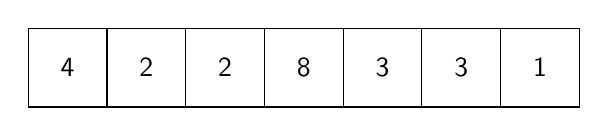
\begin{tikzpicture}[node distance=0cm, font=\sffamily, every node/.style={minimum width=1cm, minimum height=1cm, outer sep=0pt, anchor = west}, line join=miter, line cap=rect]
        \node[draw, fill=white] at (1, 0) {4};
        \node[draw, fill=white] at (2, 0) {2};
        \node[draw, fill=white] at (3, 0) {2};
        \node[draw, fill=white] at (4, 0) {8};
        \node[draw, fill=white] at (5, 0) {3};
        \node[draw, fill=white] at (6, 0) {3};
        \node[draw, fill=white] at (7, 0) {1};
    \end{tikzpicture}
\end{center}

\textbf{Bước 1:} Tìm $min$ và $max$ trong mảng để tính $k = max - min + 1
= 8 - 1 + 1 = 8$. Khởi tạo mảng đếm $count$ có kích thước $k$:

\begin{center}
    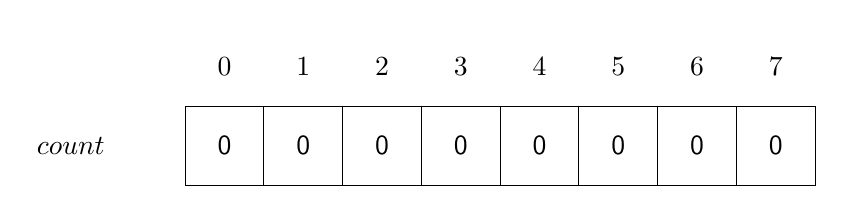
\begin{tikzpicture}[node distance=0cm, font=\sffamily, every node/.style={minimum width=1cm, minimum height=1cm, outer sep=0pt, anchor = west}, line join=miter, line cap=rect]
        \node[font=\rmfamily] at (2, 0) {0};
        \node[font=\rmfamily] at (3, 0) {1};
        \node[font=\rmfamily] at (4, 0) {2};
        \node[font=\rmfamily] at (5, 0) {3};
        \node[font=\rmfamily] at (6, 0) {4};
        \node[font=\rmfamily] at (7, 0) {5};
        \node[font=\rmfamily] at (8, 0) {6};
        \node[font=\rmfamily] at (9, 0) {7};
		\node[font=\rmfamily] at (0, -1) {$count$};
        \node[draw, fill=white] at (2, -1) {0};
        \node[draw, fill=white] at (3, -1) {0};
        \node[draw, fill=white] at (4, -1) {0};
        \node[draw, fill=white] at (5, -1) {0};
        \node[draw, fill=white] at (6, -1) {0};
        \node[draw, fill=white] at (7, -1) {0};
        \node[draw, fill=white] at (8, -1) {0};
        \node[draw, fill=white] at (9, -1) {0};
    \end{tikzpicture}
\end{center}

\textbf{Bước 2:} Duyệt qua từng phần tử trong mảng để đếm số lần xuất hiện
và lưu vào mảng đếm $(count)$ tại vị trí tương ứng với giá trị của phần tử 
đó trừ đi giá trị nhỏ nhất trong mảng đầu vào. Khi đó sẽ thu được mảng:

\begin{center}
    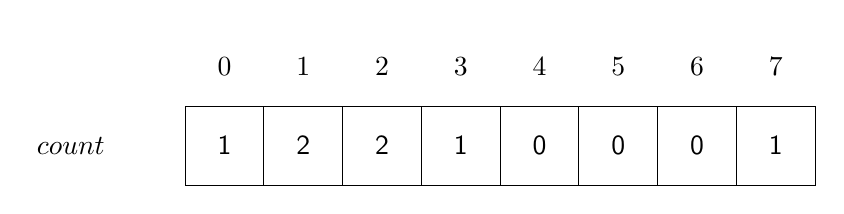
\begin{tikzpicture}[node distance=0cm, font=\sffamily, every node/.style={minimum width=1cm, minimum height=1cm, outer sep=0pt, anchor = west}, line join=miter, line cap=rect]
        \node[font=\rmfamily] at (2, 0) {0};
        \node[font=\rmfamily] at (3, 0) {1};
        \node[font=\rmfamily] at (4, 0) {2};
        \node[font=\rmfamily] at (5, 0) {3};
        \node[font=\rmfamily] at (6, 0) {4};
        \node[font=\rmfamily] at (7, 0) {5};
        \node[font=\rmfamily] at (8, 0) {6};
        \node[font=\rmfamily] at (9, 0) {7};
		\node[font=\rmfamily] at (0, -1) {$count$};
        \node[draw, fill=white] at (2, -1) {1};
        \node[draw, fill=white] at (3, -1) {2};
        \node[draw, fill=white] at (4, -1) {2};
        \node[draw, fill=white] at (5, -1) {1};
        \node[draw, fill=white] at (6, -1) {0};
        \node[draw, fill=white] at (7, -1) {0};
        \node[draw, fill=white] at (8, -1) {0};
        \node[draw, fill=white] at (9, -1) {1};
    \end{tikzpicture}
\end{center}

\textbf{Bước 3:} Tính tổng tích lũy cho mảng đếm $(count)$ sẽ thu được mảng sau:

\begin{center}
    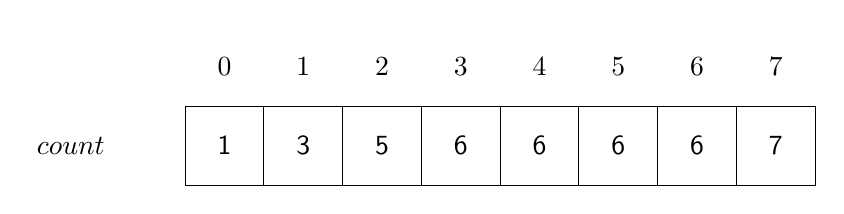
\begin{tikzpicture}[node distance=0cm, font=\sffamily, every node/.style={minimum width=1cm, minimum height=1cm, outer sep=0pt, anchor = west}, line join=miter, line cap=rect]
        \node[font=\rmfamily] at (2, 0) {0};
        \node[font=\rmfamily] at (3, 0) {1};
        \node[font=\rmfamily] at (4, 0) {2};
        \node[font=\rmfamily] at (5, 0) {3};
        \node[font=\rmfamily] at (6, 0) {4};
        \node[font=\rmfamily] at (7, 0) {5};
        \node[font=\rmfamily] at (8, 0) {6};
        \node[font=\rmfamily] at (9, 0) {7};
		\node[font=\rmfamily] at (0, -1) {$count$};
        \node[draw, fill=white] at (2, -1) {1};
        \node[draw, fill=white] at (3, -1) {3};
        \node[draw, fill=white] at (4, -1) {5};
        \node[draw, fill=white] at (5, -1) {6};
        \node[draw, fill=white] at (6, -1) {6};
        \node[draw, fill=white] at (7, -1) {6};
        \node[draw, fill=white] at (8, -1) {6};
        \node[draw, fill=white] at (9, -1) {7};
    \end{tikzpicture}
\end{center}

\textbf{Bước 4:} Xây dựng mảng kết quả theo công thức 
$output[count[input[i] - min] - 1] = input[i]$ và giảm giá trị mảng đếm
tại vị trí vừa truy cập. Khi đó ta được mảng đã sắp xếp:

\begin{center}
    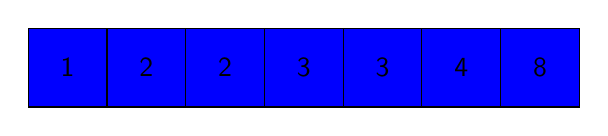
\begin{tikzpicture}[node distance=0cm, font=\sffamily, every node/.style={minimum width=1cm, minimum height=1cm, outer sep=0pt, anchor = west}, line join=miter, line cap=rect]
        \node[draw, fill=blue] at (1, 0) {1};
        \node[draw, fill=blue] at (2, 0) {2};
        \node[draw, fill=blue] at (3, 0) {2};
        \node[draw, fill=blue] at (4, 0) {3};
        \node[draw, fill=blue] at (5, 0) {3};
        \node[draw, fill=blue] at (6, 0) {4};
        \node[draw, fill=blue] at (7, 0) {8};
    \end{tikzpicture}
\end{center}

\subsubsection{Độ phức tạp thuật toán}

Với $k$ là giá trị lớn nhất trong mảng trừ giá trị nhỏ nhất cộng thêm 1. Ta có:

\begin{itemize}
	\item Độ phức tạp thời gian \cite[p.~209]{cormen2022}
	\begin{itemize}[label=$\circ$]
		\item Trường hợp tốt nhất: $O\left(n+k\right)$. Khi khi $k$ nhỏ 
		(các giá trị trong mảng nằm trong một khoảng hẹp), Counting Sort 
		chỉ cần thực hiện một số ít phép đếm và truy cập mảng đếm.
		\item Trường hợp xấu nhất: $O\left(n+k\right)$. Khi $k$ lớn (các 
		giá trị trong mảng nằm trong một khoảng rất rộng), thuật toán 
		vẫn phải tạo và xử lý mảng đếm có kích thước $k$.
		\item Trường hợp trung bình: $O\left(n+k\right)$. Trong mọi 
		trường hợp, Counting Sort luôn thực hiện một số bước cố định: 
		đếm số lần xuất hiện, tính tổng tích lũy và xây dựng mảng kết quả. 
		Do đó, độ phức tạp trung bình cũng là $O\left(n+k\right)$. 
	\end{itemize}
	\item Độ phức tạp không gian: $O\left(n+k\right)$. Counting Sort 
	yêu cầu thêm không gian để lưu trữ:
	\begin{itemize}[label=$\circ$]
		\item Mảng đếm: Có kích thước $k$ để đếm số lần xuất hiện của 
		các giá trị trong mảng đầu vào.
		\item Mảng kết quả: Có kích thước $n$ để lưu trữ mảng đã sắp xếp.
	\end{itemize}
\end{itemize}
\subsection{Shaker Sort}

\subsubsection{Ý tưởng}

Shaker Sort là một biến thể của Bubble Sort, trong đó việc duyệt mảng được thực hiện theo cả hai chiều (trái sang phải và ngược lại). Điều này giúp giảm số lần duyệt trong trường hợp các phần tử lớn đã nằm ở cuối mảng.

\subsubsection{Mã giả}

\begin{algorithm}[H]
	\caption{Shaker Sort}
	\label{shaker-sort}
	
	\SetKwFunction{ShakerSort}{ShakerSort}
	\SetKwFunction{Shaker Sort}{Shaker Sort}
	\SetKwProg{Fn}{Function}{:}{}
	\Fn{\ShakerSort {arr\KwSty{[ ]}, n}}{
		$left \gets 0$ \\
		$right \gets n - 1$  \\
		
		\While{$left < right$}{
			\For{$i = left$ \KwTo $right - 1$}{
				\If{$arr[i] > arr[i+1]$}{
					swap($arr[i]$, $arr[i+1]$)
				}
			}
			$right--$ \\
			\For{$i = right - 1$ \KwSty{downto} $left$}{
				\If{$arr[i] > arr[i+1]$}{
					swap($arr[i]$, $arr[i+1]$)
				}
			}
			$left++$
		}
	}
	\textbf{end function}
\end{algorithm}

\subsubsection{Ví dụ}

\subsubsection{Độ phức tạp thuật toán}

\begin{itemize}
	\item Độ phức tạp thời gian
	\begin{itemize}[label=$\circ$]
		\item Trường hợp tốt nhất: $O\left(n\right)$. Khi mảng đầu vào đã được sắp xếp hoàn toàn. Trong lần duyệt đầu tiên (từ trái sang phải), không có hoán đổi nào xảy ra. Thuật toán nhận biết điều này thông qua một cờ hiệu (flag) và kết thúc sớm. Vì thế chỉ cần thực hiện một lần duyệt qua mảng
		\item Trường hợp xấu nhất: $O\left(n^2\right)$. Khi mảng đầu vào được sắp xếp theo thứ tự ngược hoàn toàn. Mỗi phần tử phải được hoán đổi qua lại nhiều lần để đến đúng vị trí. Trong lượt duyệt thứ $i$, thuật toán thực hiện $n - 1$ phép so sánh.
		Tổng số phép so sánh (tương tự như Bubble Sort): 
		\begin{equation*}
			\left(n-1\right)+\left(n-2\right)+\ldots+2+1=\frac{n\left(n-1\right)}{2}\approx n^2
		\end{equation*}
		\item Trường hợp trung bình: $O\left(n^2\right)$. Khi mảng đầu vào có thứ tự ngẫu nhiên. Các phần tử được hoán đổi theo cả hai chiều trong mỗi lượt duyệt. Số lượt duyệt và số phép so sánh vẫn tương tự trường hợp xấu nhất, mặc dù có thể ít hoán đổi hơn.
	\end{itemize}
	\item Độ phức tạp không gian: $O(1)$. Vì Shaker Sort là một thuật toán in-place, tức là nó không sử dụng thêm không gian phụ đáng kể ngoài các biến tạm thời ($left$ và $right$).  
\end{itemize}

\subsubsection{Các cải tiến của thuật toán}

\begin{itemize}
	\item Dừng sớm khi mảng đã sắp xếp \\
	Sử dụng một cờ hiệu (flag) để kiểm tra xem có xảy ra hoán đổi trong một lượt duyệt hay không, nếu không có hoán đổi, kết thúc sớm thay vì tiếp tục duyệt. Điều này giúp giảm số lần duyệt trong trường hợp mảng gần như đã sắp xếp.
	\item Giảm số lần so sánh \\
	Thay vì luôn duyệt đến cuối mảng, có thể ghi lại vị trí của lần hoán đổi cuối cùng. Phần sau vị trí này đã được sắp xếp và không cần kiểm tra nữa.
	\item Kết hợp với Binary Search \\
	Nếu mảng đầu vào gần như đã sắp xếp, có thể kết hợp Shaker Sort với Binary Search để tìm vị trí chính xác cho các phần tử bị sai vị trí, giảm số lần hoán đổi.
\end{itemize}
\subsection{Flash Sort}

\subsubsection{Ý tưởng}

Dựa trên phân phối, khai thác sự phân phối tự nhiên của dữ liệu đầu vào để đạt được độ phức tạp thời gian tuyến tính $O\left(n\right)$ cho dữ liệu phân phối đồng đều. Bao gồm 3 phần chính: phân loại, hoán vị và chèn trực tiếp.

\begin{itemize}
	\item Phân loại
		\begin{itemize}[label=$\circ$]
			\item Chia các phần tử thành các lớp dựa trên giá trị của chúng. 
			\item Sử dụng mối quan hệ tuyến tính giữa giá trị phần tử và vị trí của chúng. 
			\item Công thức: $class(x) = \dfrac{(m-1)(x-min)}{max-min}$
		\end{itemize}
	\item Hoán vị
		\begin{itemize}[label=$\circ$]
			\item Di chuyển các phần tử đến vị trí gần đúng của chúng. 
			\item Tạo ra sự sắp xếp sơ bộ dựa trên phân phối lớp. 
		\end{itemize}
	\item Chèn trực tiếp: Sử dụng sắp xếp chèn để sắp xếp lại lần cuối cùng.
		\begin{itemize}[label=$\circ$]
			\item Hiệu quả vì các phần tử đã gần như được sắp xếp.  
			\item Hoạt động trên các phạm vi nhỏ trong các lớp.  
		\end{itemize}
\end{itemize}

\subsubsection{Mã giả}

\begin{algorithm}[H]
	\caption{Flash Sort}
	\label{flash-sort}
	\SetKwFunction{FlashSort}{FlashSort}
	\SetKwProg{Fn}{Function}{:}{}
	\Fn{\FlashSort {arr\KwSty{[ ]}, n}}{
		// Tìm giá trị nhỏ nhất và lớn nhất trong mảng $arr$ \\
		$a\_imin = arr[0], \hspace{0.2cm} imax = 0$ \\
		\For{$i = 0$ \KwTo $n-1$}{
			\If{$arr[i] < a\_imin$}{
				$a\_imin = arr[i]$
			}
			\If{$arr[i] > arr[imax]$}{
				$imax = i$
			}
		}
		// Tính số lượng lớp cần phân loại \\
		$m = max(0.45 * n, 1)$ \\
		Khởi tạo mảng $L$ với kích thước $m$ \\
		$c1 = (m - 1.0) / (arr[imax] - a\_imin)$ \\
			\For{$i = 0$ \KwTo $n-1$}{
			$L[c1 * (arr[i] - a\_imin)]++$
		}
		\For{$i = 1$ \KwTo $m-1$}{
			$L[i] += L[i - 1]$
		}
		swap($arr[imax]$, $arr[0]$) \\
		// Hoán vị \\
		$nmove = 0, \hspace{0.2cm} j = 0, \hspace{0.2cm} k = m - 1$ \\
	}
\end{algorithm}

%----------------------------------------------------------------------

\begingroup
\renewcommand{\thealgocf}{} % Loại bỏ số thứ tự
\setlength{\algotitleheightrule}{0pt} % Loại bỏ dòng kẻ trên tiêu đề
\setlength{\interspacetitleruled}{0pt} % Không khoảng cách giữa tiêu đề và đường kẻ
\setlength{\interspacealgoruled}{0pt} % Không khoảng cách giữa đường kẻ và nội dung

\begin{algorithm}[H]
	\setcounter{AlgoLine}{24} % Tiếp tục số dòng từ phần trước
	\SetInd{1em}{1em} % Đặt khoảng thụt lề tương tự phần 1
	\SetKwProg{Fn}{}{}{} % Không hiển thị "Function" ở phần 2
	\Fn{}{% Duy trì khối thụt lề và vline
		\While{$nmove < n - 1$}{
			\While{$j > L[k] - 1$}{
				$j++$ \\
				$k = c1 * (arr[j] - a\_imin)$
			}
			$flash = arr[j]$ \\
			\While{$j != L[k]$}{
				$k = c1 * (flash - a\_imin)$ \\
				swap($flash$, $arr[L[k] - 1]$) \\
				$L[k]--, \hspace{0.2cm} nmove++$
			}
		}
		InsertionSort(a, n) \tcp{Chèn trực tiếp trên phạm vi từng lớp}
	}
	\textbf{end function}
\end{algorithm}

\subsubsection{Ví dụ}

\begin{tikzpicture}[node distance=0cm, font=\sffamily, every node/.style={minimum width=1cm, minimum height=1cm, outer sep=0pt, anchor = west}, line join=miter, line cap=rect]
	
	% Trạng thái ban đầu
	\node[font=\rmfamily] at (0, 0) {Giả sử ta có mảng ban đầu với $n=7$ như sau:};
	\node[draw, fill=white] at (9, 0) {8};
	\node[draw, fill=white] at (10, 0) {3};
	\node[draw, fill=white] at (11, 0) {1};
	\node[draw, fill=white] at (12, 0) {7};
	\node[draw, fill=white] at (13, 0) {0};
	\node[draw, fill=white] at (14, 0) {10};
	\node[draw, fill=white] at (15, 0) {2};
	
\end{tikzpicture}

\textbf{Bước 1:} Tìm giá trị nhỏ nhất và lớn nhất: $min=0$, $max=10$ (ở vị trí $imax=5$).

\textbf{Bước 2:} Tính được số lớp $m = max(0,45*n,1) = 3$.

Từ đó dựa vào công thức phân lớp ở phần ý tưởng, ta xác định được:

\hspace{0.5cm} $\bullet$ Lớp 0 gồm các phần tử: 3, 1, 0, 2.

\hspace{0.5cm} $\bullet$ Lớp 1 gồm các phần tử: 8, 7.

\hspace{0.5cm} $\bullet$ Lớp 2 gồm phần tử: 10.

\begin{tikzpicture}[node distance=0cm, font=\sffamily, every node/.style={minimum width=1cm, minimum height=1cm, outer sep=0pt, anchor = west}, line join=miter, line cap=rect]
	
	% Trạng thái ban đầu
	\node[font=\rmfamily] at (0, -0.5) {{\bfseries Bước 3:} Hoán vị $a[imax]$ với $a[0]$ được:};
	\node[draw, fill=yellow] at (9, -0.4) {10};
	\node[draw, fill=white] at (10, -0.4) {3};
	\node[draw, fill=white] at (11, -0.4) {1};
	\node[draw, fill=white] at (12, -0.4) {7};
	\node[draw, fill=white] at (13, -0.4) {0};
	\node[draw, fill=yellow] at (14, -0.4) {8};
	\node[draw, fill=white] at (15, -0.4) {2};
	
	\node[font=\rmfamily, text width=18cm] at (0, -2) {{\bfseries Bước 4:} Phân hoạch các phần tử vào các phân vùng. Ở giai đoạn này, ta sẽ sử dụng thêm mảng $L[0..m-1]$, trong đó $L[k]-1$ sẽ chỉ vào biên bên phải của phân vùng thứ $k$.};
\end{tikzpicture}

\begin{tikzpicture}[node distance=0cm, font=\sffamily, every node/.style={minimum width=1cm, minimum height=1cm, outer sep=0pt, anchor = west}, line join=miter, line cap=rect]
	
	% Swap lần 1
	\node[font=\rmfamily] at (0, 0) {$\bullet$ Bắt đầu với $j=0$, $flash = a[j] = 10 \rightarrow$ Hoán vị $flash$ với $a[L[2] - 1]$ rồi giảm $L[2]$ đi 1 đơn vị.};
	\node[draw, fill=white] at (3, -2) {10};
	\node[draw, fill=white] at (4, -2) {3};
	\node[draw, fill=white] at (5, -2) {1};
	\node[draw, fill=white] at (6, -2) {7};
	\node[draw, fill=white] at (7, -2) {0};
	\node[draw, fill=white] at (8, -2) {8};
	\node[draw, fill=yellow] at (9, -2) {2};
	\node[draw, fill=yellow] at (11, -2) {$flash = 10$};
	\node[draw, font=\rmfamily, scale = 0.8] at (7, -0.8) {$L[2]-1$};
	\draw[->, >=stealth, line width=0.5mm, shorten <=0pt] (8.38, -0.8) -- (9.4, -1.5);
	\draw[->, >=stealth, line width=0.5mm, shorten <=0pt] (9.6, -1) -- (9.6, -1.5);
	\draw[->, >=stealth, line width=0.5mm, shorten <=0pt] (12, -1) -- (12, -1.5);
	\draw[line width=0.5mm, shorten <=0pt] (9.6, -1) -- (12, -1);
\end{tikzpicture}

\begin{tikzpicture}[node distance=0cm, font=\sffamily, every node/.style={minimum width=1cm, minimum height=1cm, outer sep=0pt, anchor = west}, line join=miter, line cap=rect]
	
	% Swap lần 2
	\node[font=\rmfamily] at (0, 0) {$\bullet$ Với $flash = 2 \rightarrow$ Hoán vị $flash$ với $a[L[0] - 1]$ rồi giảm $L[0]$ đi 1 đơn vị.};
	\node[draw, fill=white] at (3, -2) {10};
	\node[draw, fill=white] at (4, -2) {3};
	\node[draw, fill=white] at (5, -2) {1};
	\node[draw, fill=yellow] at (6, -2) {7};
	\node[draw, fill=white] at (7, -2) {0};
	\node[draw, fill=white] at (8, -2) {8};
	\node[draw, fill=blue] at (9, -2) {10};
	\node[draw, fill=yellow] at (11, -2) {$flash = 2$};
	\node[draw, font=\rmfamily, scale = 0.8] at (4, -0.8) {$L[0]-1$};
	\draw[->, >=stealth, line width=0.5mm, shorten <=0pt] (5.38, -0.8) -- (6.4, -1.5);
	\draw[->, >=stealth, line width=0.5mm, shorten <=0pt] (6.6, -1) -- (6.6, -1.5);
	\draw[->, >=stealth, line width=0.5mm, shorten <=0pt] (12, -1) -- (12, -1.5);
	\draw[line width=0.5mm, shorten <=0pt] (6.6, -1) -- (12, -1);
\end{tikzpicture}

\vspace{0.8cm}

\begin{tikzpicture}[node distance=0cm, font=\sffamily, every node/.style={minimum width=1cm, minimum height=1cm, outer sep=0pt, anchor = west}, line join=miter, line cap=rect]
	
	% Swap lần 3
	\node[font=\rmfamily] at (0, 0) {$\bullet$ Với $flash = 7 \rightarrow$ Hoán vị $flash$ với $a[L[1] - 1]$ rồi giảm $L[1]$ đi 1 đơn vị.};
	\node[draw, fill=white] at (3, -2) {10};
	\node[draw, fill=white] at (4, -2) {3};
	\node[draw, fill=white] at (5, -2) {1};
	\node[draw, fill=blue] at (6, -2) {2};
	\node[draw, fill=white] at (7, -2) {0};
	\node[draw, fill=yellow] at (8, -2) {8};
	\node[draw, fill=blue] at (9, -2) {10};
	\node[draw, fill=yellow] at (11, -2) {$flash = 7$};
	\node[draw, font=\rmfamily, scale = 0.8] at (6, -0.8) {$L[1]-1$};
	\draw[->, >=stealth, line width=0.5mm, shorten <=0pt] (7.38, -0.8) -- (8.4, -1.5);
	\draw[->, >=stealth, line width=0.5mm, shorten <=0pt] (8.6, -1) -- (8.6, -1.5);
	\draw[->, >=stealth, line width=0.5mm, shorten <=0pt] (12, -1) -- (12, -1.5);
	\draw[line width=0.5mm, shorten <=0pt] (8.6, -1) -- (12, -1);
\end{tikzpicture}

\vspace{0.8cm}

\begin{tikzpicture}[node distance=0cm, font=\sffamily, every node/.style={minimum width=1cm, minimum height=1cm, outer sep=0pt, anchor = west}, line join=miter, line cap=rect]
	
	% Swap lần 4
	\node[font=\rmfamily] at (0, 0) {$\bullet$ Với $flash = 8 \rightarrow$ Hoán vị $flash$ với $a[L[1] - 1]$ rồi giảm $L[1]$ đi 1 đơn vị.};
	\node[draw, fill=white] at (3, -2) {10};
	\node[draw, fill=white] at (4, -2) {3};
	\node[draw, fill=white] at (5, -2) {1};
	\node[draw, fill=blue] at (6, -2) {2};
	\node[draw, fill=yellow] at (7, -2) {0};
	\node[draw, fill=blue] at (8, -2) {7};
	\node[draw, fill=blue] at (9, -2) {10};
	\node[draw, fill=yellow] at (11, -2) {$flash = 8$};
	\node[draw, font=\rmfamily, scale = 0.8] at (5, -0.8) {$L[1]-1$};
	\draw[->, >=stealth, line width=0.5mm, shorten <=0pt] (6.38, -0.8) -- (7.4, -1.5);
	\draw[->, >=stealth, line width=0.5mm, shorten <=0pt] (7.6, -1) -- (7.6, -1.5);
	\draw[->, >=stealth, line width=0.5mm, shorten <=0pt] (12, -1) -- (12, -1.5);
	\draw[line width=0.5mm, shorten <=0pt] (7.6, -1) -- (12, -1);
\end{tikzpicture}

\vspace{0.8cm}

\begin{tikzpicture}[node distance=0cm, font=\sffamily, every node/.style={minimum width=1cm, minimum height=1cm, outer sep=0pt, anchor = west}, line join=miter, line cap=rect]
	
	% Swap lần 5
	\node[font=\rmfamily] at (0, 0) {$\bullet$ Với $flash = 0 \rightarrow$ Hoán vị $flash$ với $a[L[0] - 1]$ rồi giảm $L[0]$ đi 1 đơn vị.};
	\node[draw, fill=white] at (3, -2) {10};
	\node[draw, fill=white] at (4, -2) {3};
	\node[draw, fill=yellow] at (5, -2) {1};
	\node[draw, fill=blue] at (6, -2) {2};
	\node[draw, fill=blue] at (7, -2) {8};
	\node[draw, fill=blue] at (8, -2) {7};
	\node[draw, fill=blue] at (9, -2) {10};
	\node[draw, fill=yellow] at (11, -2) {$flash = 0$};
	\node[draw, font=\rmfamily, scale = 0.8] at (3, -0.8) {$L[0]-1$};
	\draw[->, >=stealth, line width=0.5mm, shorten <=0pt] (4.38, -0.8) -- (5.4, -1.5);
	\draw[->, >=stealth, line width=0.5mm, shorten <=0pt] (5.6, -1) -- (5.6, -1.5);
	\draw[->, >=stealth, line width=0.5mm, shorten <=0pt] (12, -1) -- (12, -1.5);
	\draw[line width=0.5mm, shorten <=0pt] (5.6, -1) -- (12, -1);
\end{tikzpicture}

\vspace{0.8cm}

\begin{tikzpicture}[node distance=0cm, font=\sffamily, every node/.style={minimum width=1cm, minimum height=1cm, outer sep=0pt, anchor = west}, line join=miter, line cap=rect]
	
	% Swap lần 6
	\node[font=\rmfamily] at (0, 0) {$\bullet$ Với $flash = 1 \rightarrow$ Hoán vị $flash$ với $a[L[0] - 1]$ rồi giảm $L[0]$ đi 1 đơn vị.};
	\node[draw, fill=white] at (3, -2) {10};
	\node[draw, fill=yellow] at (4, -2) {3};
	\node[draw, fill=blue] at (5, -2) {0};
	\node[draw, fill=blue] at (6, -2) {2};
	\node[draw, fill=blue] at (7, -2) {8};
	\node[draw, fill=blue] at (8, -2) {7};
	\node[draw, fill=blue] at (9, -2) {10};
	\node[draw, fill=yellow] at (11, -2) {$flash = 1$};
	\node[draw, font=\rmfamily, scale = 0.8] at (2, -0.8) {$L[0]-1$};
	\draw[->, >=stealth, line width=0.5mm, shorten <=0pt] (3.38, -0.8) -- (4.4, -1.5);
	\draw[->, >=stealth, line width=0.5mm, shorten <=0pt] (4.6, -1) -- (4.6, -1.5);
	\draw[->, >=stealth, line width=0.5mm, shorten <=0pt] (12, -1) -- (12, -1.5);
	\draw[line width=0.5mm, shorten <=0pt] (4.6, -1) -- (12, -1);
\end{tikzpicture}


\vspace{0.8cm}

\begin{tikzpicture}[node distance=0cm, font=\sffamily, every node/.style={minimum width=1cm, minimum height=1cm, outer sep=0pt, anchor = west}, line join=miter, line cap=rect]
	
	% Swap lần 7
	\node[font=\rmfamily] at (0, 0) {$\bullet$ Với $flash = 3 \rightarrow$ Hoán vị $flash$ với $a[L[0] - 1]$ rồi giảm $L[0]$ đi 1 đơn vị.};
	\node[draw, fill=yellow] at (3, -2) {10};
	\node[draw, fill=blue] at (4, -2) {1};
	\node[draw, fill=blue] at (5, -2) {0};
	\node[draw, fill=blue] at (6, -2) {2};
	\node[draw, fill=blue] at (7, -2) {8};
	\node[draw, fill=blue] at (8, -2) {7};
	\node[draw, fill=blue] at (9, -2) {10};
	\node[draw, fill=yellow] at (11, -2) {$flash = 3$};
	\node[draw, font=\rmfamily, scale = 0.8] at (1, -0.8) {$L[0]-1$};
	\draw[->, >=stealth, line width=0.5mm, shorten <=0pt] (2.38, -0.8) -- (3.4, -1.5);
	\draw[->, >=stealth, line width=0.5mm, shorten <=0pt] (3.6, -1) -- (3.6, -1.5);
	\draw[->, >=stealth, line width=0.5mm, shorten <=0pt] (12, -1) -- (12, -1.5);
	\draw[line width=0.5mm, shorten <=0pt] (3.6, -1) -- (12, -1);
	
	%Phân hoạch xong
	% Swap lần 7
	\node[font=\rmfamily] at (0, -3) {$\bullet$ Như vậy sau bước này, các phần tử đã được đưa về đúng phân vùng của nó:};
	\node[draw, fill=blue] at (3, -4) {3};
	\node[draw, fill=blue] at (4, -4) {1};
	\node[draw, fill=blue] at (5, -4) {0};
	\node[draw, fill=blue] at (6, -4) {2};
	\node[draw, fill=blue] at (7, -4) {8};
	\node[draw, fill=blue] at (8, -4) {7};
	\node[draw, fill=blue] at (9, -4) {10};
	
	% Sắp xếp xong
	\node[font=\rmfamily] at (0, -5.3) {{\bfseries Bước 5:} Cuối cùng, ở mỗi phân vùng, sử dụng Insertion Sort để đưa các phần tử về đúng vị trí.};
\end{tikzpicture}

\subsubsection{Độ phức tạp thuật toán}

\begin{itemize}
	\item Độ phức tạp thời gian
	\begin{itemize}[label=$\circ$]
		\item Trường hợp tốt nhất: $O\left(n\right)$. Khi mảng đầu vào có các phần tử 
		phân bố đều, và số lượng lớp được chọn hợp lý. Trong trường hợp 
		này, các phần tử được phân phối đều giữa các lớp, giảm tối đa số 
		lần hoán đổi. Việc sắp xếp trong mỗi lớp bằng Insertion Sort được 
		thực hiện nhanh chóng do số phần tử trong mỗi lớp nhỏ. Tất cả các 
		bước chính (phân loại, hoán vị và chèn trực tiếp) đều có độ phức 
		tạp là $O\left(n\right)$.
		\item Trường hợp xấu nhất: $O\left(n^2\right)$. Khi các phần tử trong mảng phân 
		phối không đều hoặc số lượng lớp được chọn không hợp lý. Khi đó, một 
		số lớp có thể chứa nhiều phần tử, dẫn đến việc sắp xếp trong lớp trở 
		thành $O\left(k^2\right)$, với $k$ là số phần tử trong lớp lớn nhất. Nếu số lượng 
		lớp quá nhỏ, thuật toán mất lợi thế phân chia và gần như phải sắp xếp 
		toàn bộ mảng trong một lớp lớn.
		\item Trường hợp trung bình: $O\left(n\right)$. Trong trường hợp này, các phần 
		tử được phân phối đủ đều giữa các lớp và việc sắp xếp trong lớp 
		diễn ra hiệu quả. Thuật toán duy trì độ phức tạp tuyến tính trong 
		cả ba bước (phân loại, hoán vị và chèn trực tiếp).
	\end{itemize}
	
	\item Độ phức tạp không gian: $O\left(n\right)$. Flash Sort yêu cầu không gian 
	phụ để lưu mảng lớp, với kích thước bằng số lượng lớp $(m)$. Trong 
	trường hợp điển hình, $m \approx n/2$, dẫn đến độ phức tạp không gian 
	là $O\left(n\right)$.
\end{itemize}
\pagebreak

\section{Kết quả thực nghiệm và nhận xét}

\subsection{Kết quả thực nghiệm}

\subsubsection{Đầu vào có thứ tự ngẫu nhiên}

\begin{table}[H] % Use [H] to force the table to be placed here
    \centering
    \caption{Kết quả thực nghiệm với đầu vào có thứ tự ngẫu nhiên (Nhóm 1)}
    \begin{tblr}{
      column{even} = {r},
      column{3} = {r},
      column{5} = {r},
      column{7} = {r},
      cell{1}{2} = {c=2}{c},
      cell{1}{4} = {c=2}{c},
      cell{1}{6} = {c=2}{c},
      cell{2}{2} = {c},
      cell{2}{3} = {c},
      cell{2}{4} = {c},
      cell{2}{5} = {c},
      cell{2}{6} = {c},
      cell{2}{7} = {c},
      hline{1,3,14} = {-}{},
      hline{2} = {2-7}{},
    }
        \textbf{Data size} & \textbf{10,000} &                      & \textbf{30,000} &                      & \textbf{50,000} &                      \\
        \textbf{Metrics}   & \textbf{Time}   & \textbf{Comparisons} & \textbf{Time}   & \textbf{Comparisons} & \textbf{Time}   & \textbf{Comparisons} \\
        Selection Sort     & 110             & 100009999            & 870             & 900029999            & 2474            & 2500049999           \\
        Insertion Sort     & 58              & 49852722             & 504             & 450424387            & 1481            & 1244875082           \\
        Shell Sort         & 271             & 100009999            & 2692            & 900029999            & 7542            & 2500049999           \\
        Bubble Sort        & 268             & 100009999            & 2639            & 900029999            & 7491            & 2500049999           \\
        Heap Sort          & 1               & 638425               & 6               & 2150786              & 10              & 3771772              \\
        Merge Sort         & 3               & 583832               & 9               & 1937240              & 15              & 3383319              \\
        Quick Sort         & 1               & 276045               & 5               & 916849               & 6               & 1636700              \\
        Radix Sort         & 0               & 140056               & 1               & 510070               & 2               & 850070               \\
        Counting Sort      & 0               & 80000                & 0               & 240000               & 0               & 382769               \\
        Shaker Sort        & 219             & 75877345             & 1986            & 678034901            & 5519            & 1868558231           \\
        Flash Sort         & 0               & 97658                & 0               & 285201               & 1               & 451390
    \end{tblr}
\end{table}

\begin{table}[H] % Use [H] to force the table to be placed here
    \centering
    \caption{Kết quả thực nghiệm với đầu vào có thứ tự ngẫu nhiên (Nhóm 2)}
    \begin{tblr}{
      column{even} = {r},
      column{3} = {r},
      column{5} = {r},
      column{7} = {r},
      cell{1}{2} = {c=2}{c},
      cell{1}{4} = {c=2}{c},
      cell{1}{6} = {c=2}{c},
      cell{2}{2} = {c},
      cell{2}{3} = {c},
      cell{2}{4} = {c},
      cell{2}{5} = {c},
      cell{2}{6} = {c},
      cell{2}{7} = {c},
      hline{1,3,14} = {-}{},
      hline{2} = {2-7}{},
    }
        \textbf{Data size} & \textbf{100,000} &                      & \textbf{300,000} &                      & \textbf{500,000} &                      \\
        \textbf{Metrics}   & \textbf{Time}    & \textbf{Comparisons} & \textbf{Time}    & \textbf{Comparisons} & \textbf{Time}    & \textbf{Comparisons} \\
        Selection Sort     & 10378            & 10000099999          & 91156            & 90000299999          & 306006           & 250000499999         \\
        Insertion Sort     & 5879             & 5026592949           & 68865            & 44937080911          & 231821           & 125044404674         \\
        Shell Sort         & 30370            & 10000099999          & 396729           & 90000299999          & 1182221          & 250000499999         \\
        Bubble Sort        & 31385            & 10000099999          & 454882           & 90000299999          & 1203413          & 250000499999         \\
        Heap Sort          & 21               & 8044992              & 79               & 26487787             & 140              & 45972193             \\
        Merge Sort         & 31               & 7166010              & 103              & 23383601             & 180              & 40383061             \\
        Quick Sort         & 11               & 3341712              & 54               & 10434674             & 112              & 18476753             \\
        Radix Sort         & 4                & 1700070              & 16               & 5100070              & 25               & 8500070              \\
        Counting Sort      & 1                & 732769               & 3                & 2132769              & 6                & 3532769              \\
        Shaker Sort        & 24340            & 7519014091           & 323182           & 67598742089          & 1018829          & 187569730819         \\
        Flash Sort         & 2                & 905677               & 7                & 2611012              & 19               & 4335083
    \end{tblr}
\end{table}

\subsubsection{Đầu vào có thứ tự gần được sắp xếp}

\begin{table}[H] % Use [H] to force the table to be placed here
    \centering
    \caption{Kết quả thực nghiệm với đầu vào có thứ tự gần được sắp xếp (Nhóm 1)}
    \begin{tblr}{
      column{even} = {r},
      column{3} = {r},
      column{5} = {r},
      column{7} = {r},
      cell{1}{2} = {c=2}{c},
      cell{1}{4} = {c=2}{c},
      cell{1}{6} = {c=2}{c},
      cell{2}{2} = {c},
      cell{2}{3} = {c},
      cell{2}{4} = {c},
      cell{2}{5} = {c},
      cell{2}{6} = {c},
      cell{2}{7} = {c},
      hline{1,3,14} = {-}{},
      hline{2} = {2-7}{},
    }
        \textbf{Data size} & \textbf{10,000} &                      & \textbf{30,000} &                      & \textbf{50,000} &                      \\
        \textbf{Metrics}   & \textbf{Time}   & \textbf{Comparisons} & \textbf{Time}   & \textbf{Comparisons} & \textbf{Time}   & \textbf{Comparisons} \\
        Selection Sort     & 106             & 100009999            & 868             & 900029999            & 2472            & 2500049999           \\
        Insertion Sort     & 0               & 129726               & 1               & 486366               & 1               & 560354               \\
        Shell Sort         & 96              & 100009999            & 812             & 900029999            & 2290            & 2500049999           \\
        Bubble Sort        & 94              & 100009999            & 828             & 900029999            & 2259            & 2500049999           \\
        Heap Sort          & 2               & 669904               & 5               & 2236774              & 9               & 3925280              \\
        Merge Sort         & 3               & 503802               & 7               & 1637853              & 12              & 2845326              \\
        Quick Sort         & 0               & 154995               & 1               & 501973               & 2               & 913890               \\
        Radix Sort         & 0               & 140056               & 1               & 510070               & 2               & 850070               \\
        Counting Sort      & 0               & 80001                & 0               & 240001               & 0               & 400001               \\
        Shaker Sort        & 1               & 299791               & 1               & 899791               & 2               & 1299845              \\
        Flash Sort         & 0               & 118969               & 0               & 356969               & 1               & 594969
    \end{tblr}
\end{table}

\begin{table}[H] % Use [H] to force the table to be placed here
    \centering
    \caption{Kết quả thực nghiệm với đầu vào có thứ tự gần được sắp xếp (Nhóm 2)}
    \begin{tblr}{
      column{even} = {r},
      column{3} = {r},
      column{5} = {r},
      column{7} = {r},
      cell{1}{2} = {c=2}{c},
      cell{1}{4} = {c=2}{c},
      cell{1}{6} = {c=2}{c},
      cell{2}{2} = {c},
      cell{2}{3} = {c},
      cell{2}{4} = {c},
      cell{2}{5} = {c},
      cell{2}{6} = {c},
      cell{2}{7} = {c},
      hline{1,3,14} = {-}{},
      hline{2} = {2-7}{},
    }
        \textbf{Data size} & \textbf{100,000} &                      & \textbf{300,000} &                      & \textbf{500,000} &                      \\
        \textbf{Metrics}   & \textbf{Time}    & \textbf{Comparisons} & \textbf{Time}    & \textbf{Comparisons} & \textbf{Time}    & \textbf{Comparisons} \\
        Selection Sort     & 11396            & 10000099999          & 137957           & 90000299999          & 1295243          & 250000499999         \\
        Insertion Sort     & 1                & 706102               & 2                & 1188582              & 2                & 1905186              \\
        Shell Sort         & 9538             & 10000099999          & 166585           & 90000299999          & 1319995          & 250000499999         \\
        Bubble Sort        & 9164             & 10000099999          & 135698           & 90000299999          & 1486996          & 250000499999         \\
        Heap Sort          & 17               & 8364715              & 57               & 27413296             & 104              & 47405047             \\
        Merge Sort         & 23               & 5851166              & 95               & 18733795             & 130              & 32137705             \\
        Quick Sort         & 5                & 1927723              & 13               & 6058264              & 28               & 10310769             \\
        Radix Sort         & 4                & 1700070              & 19               & 6000084              & 26               & 10000084             \\
        Counting Sort      & 1                & 800001               & 4                & 2400001              & 6                & 4000001              \\
        Shaker Sort        & 4                & 2999791              & 7                & 6599891              & 14               & 12999845             \\
        Flash Sort         & 2                & 1189967              & 6                & 3569970              & 13               & 5949970
    \end{tblr}
\end{table}

\subsubsection{Đầu vào có thứ tự đã được sắp xếp}

\begin{table}[H] % Use [H] to force the table to be placed here
    \centering
    \caption{Kết quả thực nghiệm với đầu vào có thứ tự đã được sắp xếp (Nhóm 1)}
    \begin{tblr}{
      column{even} = {r},
      column{3} = {r},
      column{5} = {r},
      column{7} = {r},
      cell{1}{2} = {c=2}{c},
      cell{1}{4} = {c=2}{c},
      cell{1}{6} = {c=2}{c},
      cell{2}{2} = {c},
      cell{2}{3} = {c},
      cell{2}{4} = {c},
      cell{2}{5} = {c},
      cell{2}{6} = {c},
      cell{2}{7} = {c},
      hline{1,3,14} = {-}{},
      hline{2} = {2-7}{},
    }
        \textbf{Data size} & \textbf{10,000} &                      & \textbf{30,000} &                      & \textbf{50,000} &                      \\
        \textbf{Metrics}   & \textbf{Time}   & \textbf{Comparisons} & \textbf{Time}   & \textbf{Comparisons} & \textbf{Time}   & \textbf{Comparisons} \\
        Selection Sort     & 182             & 100009999            & 1426            & 900029999            & 4059            & 2500049999           \\
        Insertion Sort     & 0               & 29998                & 0               & 89998                & 0               & 149998               \\
        Shell Sort         & 179             & 100009999            & 1349            & 900029999            & 3786            & 2500049999           \\
        Bubble Sort        & 180             & 100009999            & 1346            & 900029999            & 3636            & 2500049999           \\
        Heap Sort          & 7               & 670329               & 13              & 2236648              & 18              & 3925351              \\
        Merge Sort         & 5               & 475242               & 17              & 1559914              & 25              & 2722826              \\
        Quick Sort         & 0               & 154959               & 3               & 501929               & 4               & 913850               \\
        Radix Sort         & 1               & 140056               & 2               & 510070               & 4               & 850070               \\
        Counting Sort      & 0               & 80001                & 1               & 240001               & 1               & 400001               \\
        Shaker Sort        & 0               & 20001                & 0               & 60001                & 0               & 100001               \\
        Flash Sort         & 0               & 118993               & 1               & 356993               & 2               & 594993
    \end{tblr}
\end{table}

\begin{table}[H] % Use [H] to force the table to be placed here
    \centering
    \caption{Kết quả thực nghiệm với đầu vào có thứ tự đã được sắp xếp (Nhóm 2)}
    \begin{tblr}{
      column{even} = {r},
      column{3} = {r},
      column{5} = {r},
      column{7} = {r},
      cell{1}{2} = {c=2}{c},
      cell{1}{4} = {c=2}{c},
      cell{1}{6} = {c=2}{c},
      cell{2}{2} = {c},
      cell{2}{3} = {c},
      cell{2}{4} = {c},
      cell{2}{5} = {c},
      cell{2}{6} = {c},
      cell{2}{7} = {c},
      hline{1,3,14} = {-}{},
      hline{2} = {2-7}{},
    }
        \textbf{Data size} & \textbf{100,000} &                      & \textbf{300,000} &                      & \textbf{500,000} &                      \\
        \textbf{Metrics}   & \textbf{Time}    & \textbf{Comparisons} & \textbf{Time}    & \textbf{Comparisons} & \textbf{Time}    & \textbf{Comparisons} \\
        Selection Sort     & 29478            & 10000099999          & 111585           & 90000299999          & 396841           & 250000499999         \\
        Insertion Sort     & 0                & 299998               & 3                & 899998               & 3                & 1499998              \\
        Shell Sort         & 29503            & 10000099999          & 106498           & 90000299999          & 412844           & 250000499999         \\
        Bubble Sort        & 30120            & 10000099999          & 107040           & 90000299999          & 384574           & 250000499999         \\
        Heap Sort          & 39               & 8365080              & 120              & 27413230             & 165              & 47404886             \\
        Merge Sort         & 47               & 5745658              & 137              & 18645946             & 200              & 32017850             \\
        Quick Sort         & 5                & 1927691              & 17               & 6058228              & 23               & 10310733             \\
        Radix Sort         & 9                & 1700070              & 29               & 6000084              & 56               & 10000084             \\
        Counting Sort      & 3                & 800001               & 9                & 2400001              & 14               & 4000001              \\
        Shaker Sort        & 0                & 200001               & 1                & 600001               & 2                & 1000001              \\
        Flash Sort         & 5                & 1189993              & 15               & 3569993              & 25               & 5949993
    \end{tblr}
\end{table}

\subsubsection{Đầu vào có thứ tự được sắp xếp ngược}

\begin{table}[H] % Use [H] to force the table to be placed here
    \centering
    \caption{Kết quả thực nghiệm với đầu vào có thứ tự được sắp xếp ngược (Nhóm 1)}
    \begin{tblr}{
      column{even} = {r},
      column{3} = {r},
      column{5} = {r},
      column{7} = {r},
      cell{1}{2} = {c=2}{c},
      cell{1}{4} = {c=2}{c},
      cell{1}{6} = {c=2}{c},
      cell{2}{2} = {c},
      cell{2}{3} = {c},
      cell{2}{4} = {c},
      cell{2}{5} = {c},
      cell{2}{6} = {c},
      cell{2}{7} = {c},
      hline{1,3,14} = {-}{},
      hline{2} = {2-7}{},
    }
        \textbf{Data size} & \textbf{10,000} &                      & \textbf{30,000} &                      & \textbf{50,000} &                      \\
        \textbf{Metrics}   & \textbf{Time}   & \textbf{Comparisons} & \textbf{Time}   & \textbf{Comparisons} & \textbf{Time}   & \textbf{Comparisons} \\
        Selection Sort     & 175             & 100009999            & 1477            & 900029999            & 3924            & 2500049999           \\
        Insertion Sort     & 202             & 100009999            & 1630            & 900029999            & 4686            & 2500049999           \\
        Shell Sort         & 383             & 100009999            & 3158            & 900029999            & 9485            & 2500049999           \\
        Bubble Sort        & 373             & 100009999            & 3116            & 900029999            & 9043            & 2500049999           \\
        Heap Sort          & 3               & 606771               & 10              & 2063324              & 18              & 3612724              \\
        Merge Sort         & 4               & 476441               & 16              & 1573465              & 25              & 2733945              \\
        Quick Sort         & 0               & 164975               & 1               & 531939               & 2               & 963861               \\
        Radix Sort         & 0               & 140056               & 2               & 510070               & 4               & 850070               \\
        Counting Sort      & 0               & 80001                & 1               & 240001               & 1               & 400001               \\
        Shaker Sort        & 385             & 100010001            & 3255            & 900030001            & 9005            & 2500050001           \\
        Flash Sort         & 0               & 103751               & 1               & 311251               & 2               & 518751
    \end{tblr}
\end{table}

\begin{table}[H] % Use [H] to force the table to be placed here
    \centering
    \caption{Kết quả thực nghiệm với đầu vào có thứ tự được sắp xếp ngược (Nhóm 2)}
    \begin{tblr}{
      column{even} = {r},
      column{3} = {r},
      column{5} = {r},
      column{7} = {r},
      cell{1}{2} = {c=2}{c},
      cell{1}{4} = {c=2}{c},
      cell{1}{6} = {c=2}{c},
      cell{2}{2} = {c},
      cell{2}{3} = {c},
      cell{2}{4} = {c},
      cell{2}{5} = {c},
      cell{2}{6} = {c},
      cell{2}{7} = {c},
      hline{1,3,14} = {-}{},
      hline{2} = {2-7}{},
    }
        \textbf{Data size} & \textbf{100,000} &                      & \textbf{300,000} &                      & \textbf{500,000} &                      \\
        \textbf{Metrics}   & \textbf{Time}    & \textbf{Comparisons} & \textbf{Time}    & \textbf{Comparisons} & \textbf{Time}    & \textbf{Comparisons} \\
        Selection Sort     & 10289            & 10000099999          & 149091           & 90000299999          & 286666           & 250000499999         \\
        Insertion Sort     & 12560            & 10000099999          & 161038           & 90000299999          & 335113           & 250000499999         \\
        Shell Sort         & 23060            & 10000099999          & 334815           & 90000299999          & 605040           & 250000499999         \\
        Bubble Sort        & 32013            & 10000099999          & 334914           & 90000299999          & 606656           & 250000499999         \\
        Heap Sort          & 17               & 7718943              & 59               & 25569379             & 119              & 44483348             \\
        Merge Sort         & 32               & 5767897              & 81               & 18708313             & 123              & 32336409             \\
        Quick Sort         & 5                & 2027703              & 8                & 6358249              & 16               & 10810747             \\
        Radix Sort         & 9                & 1700070              & 15               & 6000084              & 27               & 10000084             \\
        Counting Sort      & 3                & 800001               & 4                & 2400001              & 7                & 4000001              \\
        Shaker Sort        & 22892            & 10000100001          & 221549           & 90000300001          & 611441           & 250000500001         \\
        Flash Sort         & 4                & 1037501              & 8                & 3112501              & 13               & 5187501
    \end{tblr}
\end{table}

\subsection{Nhận xét}

\subsubsection{Về thời gian chạy}

$\bullet$ Với đầu vào có thứ tự ngẫu nhiên \\

\begin{figure}[H]
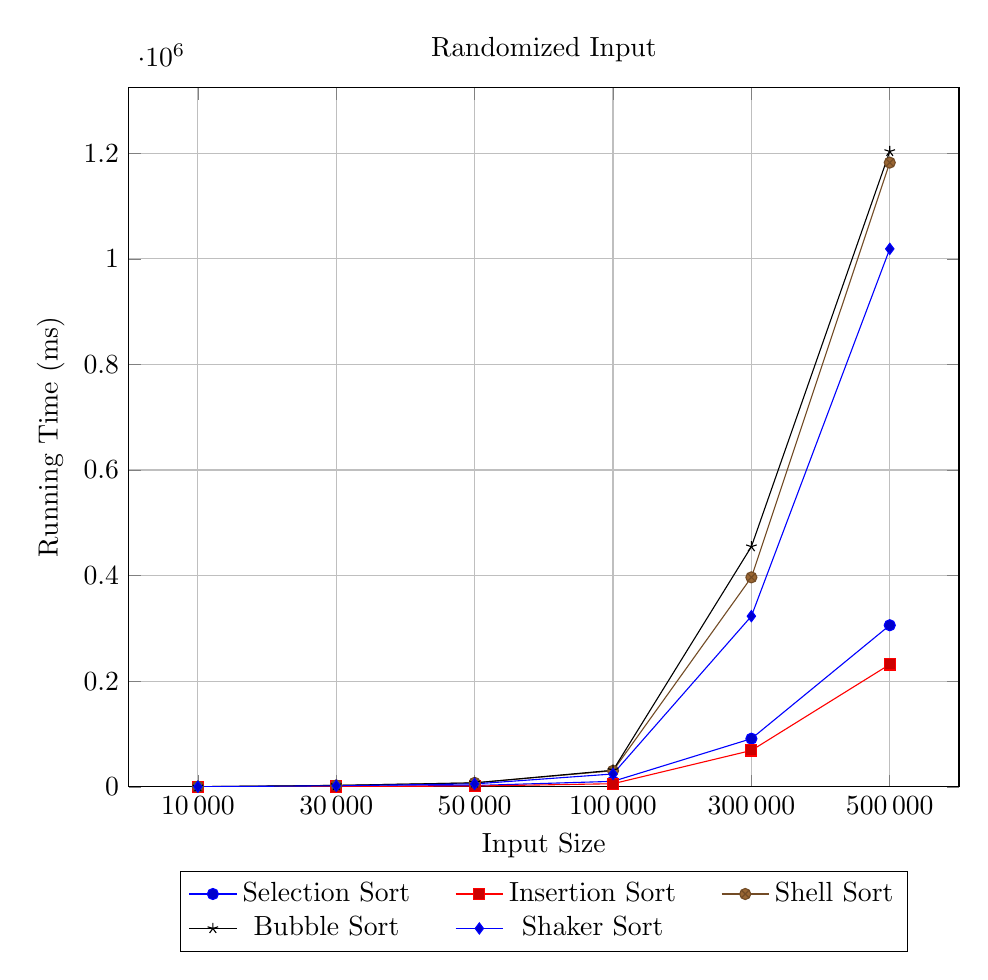
\begin{tikzpicture}
    \begin{axis}[
        width=\textwidth,
        title={Randomized Input},
        xlabel={Input Size},
        ylabel={Running Time (ms)},
        legend style={
            at={(0.5,-0.12)}, anchor=north, legend columns=3, 
            /tikz/every even column/.append style={column sep=0.5cm}
        },
        symbolic x coords={10\,000, 30\,000, 50\,000, 100\,000, 300\,000, 500\,000},
        xtick=data,
        ymin=0,
        grid=major,
    ]
    
    \addplot coordinates {(10\,000,110) (30\,000,870) (50\,000,2474) 
    (100\,000,10378) (300\,000,91156) (500\,000,306006)};
    \addlegendentry{Selection Sort}
    
    \addplot coordinates {(10\,000,58) (30\,000,504) (50\,000,1481) 
    (100\,000,5879) (300\,000,68865) (500\,000,231821)};
    \addlegendentry{Insertion Sort}
    
    \addplot coordinates {(10\,000,271) (30\,000,2692) (50\,000,7542) 
    (100\,000,30370) (300\,000,396729) (500\,000,1182221)};
    \addlegendentry{Shell Sort}
    
    \addplot coordinates {(10\,000,268) (30\,000,2639) (50\,000,7491) 
    (100\,000,31385) (300\,000,454882) (500\,000,1203413)};
    \addlegendentry{Bubble Sort}
    
    \addplot coordinates {(10\,000,219) (30\,000,1986) 
    (50\,000,5519) (100\,000,24340) (300\,000,323182) (500\,000,1018829)};
    \addlegendentry{Shaker Sort}
    
    \end{axis}
\end{tikzpicture}
\caption{Kết quả thực nghiệm với đầu vào có thứ tự ngẫu nhiên (Nhóm 1)}
\end{figure}

\begin{figure}[H]
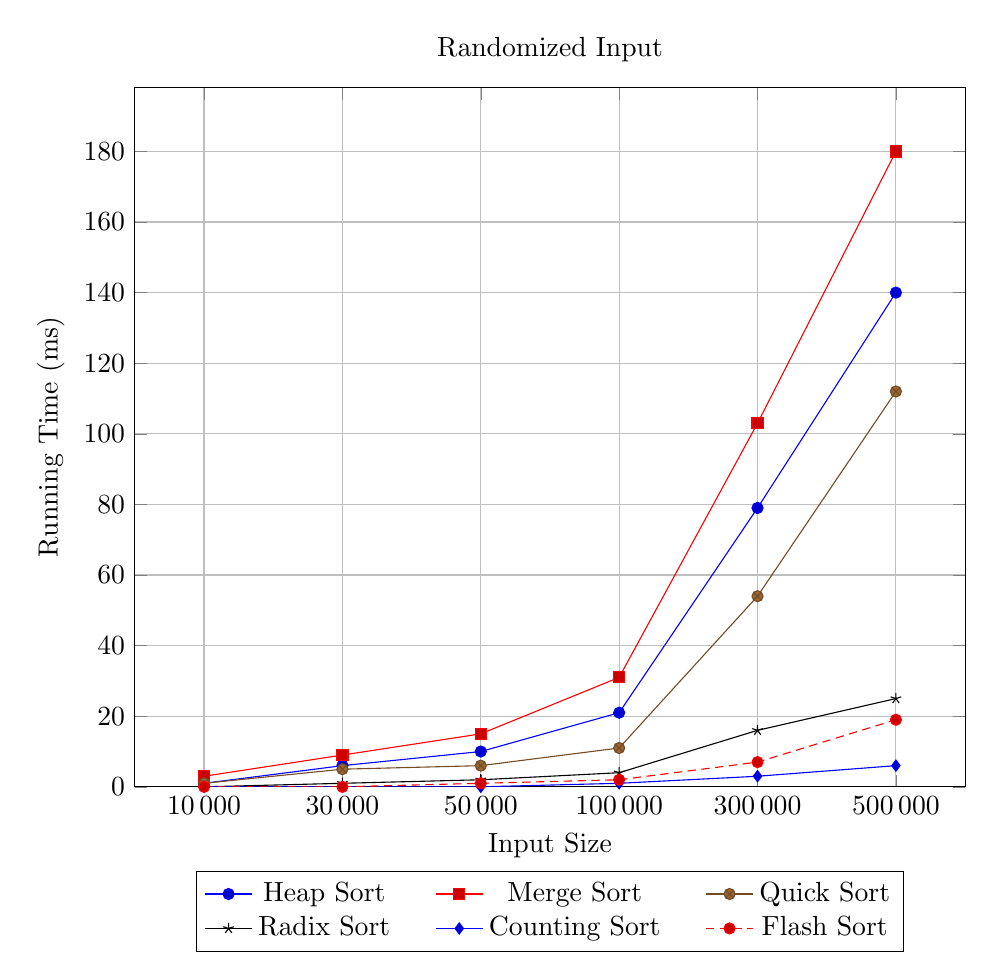
\begin{tikzpicture}
    \begin{axis}[
        width=\textwidth,
        title={Randomized Input},
        xlabel={Input Size},
        ylabel={Running Time (ms)},
        legend style={
            at={(0.5,-0.12)}, anchor=north, legend columns=3, 
            /tikz/every even column/.append style={column sep=0.5cm}
        },
        symbolic x coords={10\,000, 30\,000, 50\,000, 100\,000, 300\,000, 500\,000},
        xtick=data,
        ymin=0,
        grid=major,
    ]
    
    \addplot coordinates {(10\,000,1) (30\,000,6) (50\,000,10) 
    (100\,000,21) (300\,000,79) (500\,000,140)};
    \addlegendentry{Heap Sort}
    
    \addplot coordinates {(10\,000,3) (30\,000,9) (50\,000,15) 
    (100\,000,31) (300\,000,103) (500\,000,180)};
    \addlegendentry{Merge Sort}
    
    \addplot coordinates {(10\,000,1) (30\,000,5) (50\,000,6) 
    (100\,000,11) (300\,000,54) (500\,000,112)};
    \addlegendentry{Quick Sort}
    
    \addplot coordinates {(10\,000,0) (30\,000,1) (50\,000,2) 
    (100\,000,4) (300\,000,16) (500\,000,25)};
    \addlegendentry{Radix Sort}
    
    \addplot coordinates {(10\,000,0) (30\,000,0) (50\,000,0) 
    (100\,000,1) (300\,000,3) (500\,000,6)};
    \addlegendentry{Counting Sort}
    
    \addplot coordinates {(10\,000,0) (30\,000,0) (50\,000,1) 
    (100\,000,2) (300\,000,7) (500\,000,19)};
    \addlegendentry{Flash Sort}
    
    \end{axis}
\end{tikzpicture}
\caption{Kết quả thực nghiệm với đầu vào có thứ tự ngẫu nhiên (Nhóm 2)}
\end{figure}

\begin{itemize}[label=$\circ$]
    \item Thuật toán Bubble Sort có tốc độ chậm nhất với mọi kích thước 
    đầu vào, ngược lại Insertion Sort nhanh nhất trong nhóm thuật toán 
    có độ phức tạp là $O\left(n^2\right)$ cho dù số lượng phần tử có tăng 
    cao, thì thời gian thực thi vẫn không tăng quá nhiều. 
    \item Về nhóm thuật toán có độ phức tạp là $O\left(nlogn\right)$, 
    Merge Sort chậm đi rất nhiều khi kích thước đầu vào tăng lên do tiêu 
    tốn nhiều thời gian cho việc chia và trộn nhiều mảng con. Còn Quick 
    Sort mặc dù có tăng thời gian thực thi khi cỡ mẫu lớn hơn 100,000 
    nhưng vẫn nhanh nhất trong nhóm thuật toán này. 
    \item Cuối cùng là nhóm thuật toán có độ phức tạp là $O\left(n\right)$, 
    Counting Sort giữ vị trí thứ nhất nhưng bị hạn chế về kiểu dữ liệu, 
    như với số thực hoặc số nguyên lớn cần phải xử lý một cách khéo léo. 
    Mặc khác, Flash Sort có thể xử lý đa dạng kiểu dữ liệu và tốc độ cũng 
    đáng kể nhưng phụ thuộc vào sự phân phối của dữ liệu đầu vào và quá 
    trình cài đặt khá phức tạp.
\end{itemize}

$\bullet$ Với đầu vào có thứ tự gần được sắp xếp \\

\begin{figure}[H]
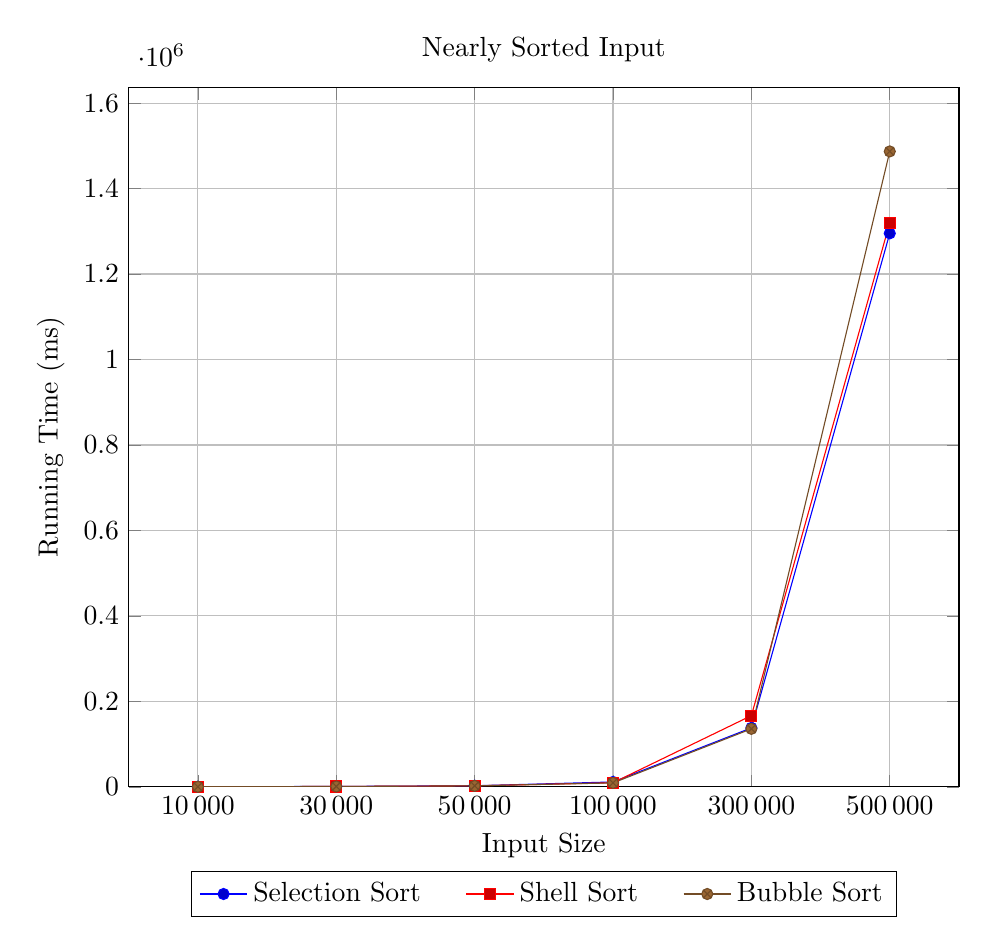
\begin{tikzpicture}
    \begin{axis}[
        width=\textwidth,
        title={Nearly Sorted Input},
        xlabel={Input Size},
        ylabel={Running Time (ms)},
        legend style={
            at={(0.5,-0.12)}, anchor=north, legend columns=3, 
            /tikz/every even column/.append style={column sep=0.5cm}
        },
        symbolic x coords={10\,000, 30\,000, 50\,000, 100\,000, 300\,000, 500\,000},
        xtick=data,
        ymin=0,
        grid=major,
    ]
    
    \addplot coordinates {(10\,000,106) (30\,000,868) (50\,000,2472) 
    (100\,000,11396) (300\,000,137957) (500\,000,1295243)};
    \addlegendentry{Selection Sort}
    
    \addplot coordinates {(10\,000,96) (30\,000,812) (50\,000,2290) 
    (100\,000,9538) (300\,000,166585) (500\,000,1319995)};
    \addlegendentry{Shell Sort}
    
    \addplot coordinates {(10\,000,94) (30\,000,828) (50\,000,2259) 
    (100\,000,9164) (300\,000,135698) (500\,000,1486996)};
    \addlegendentry{Bubble Sort}
    
    \end{axis}
\end{tikzpicture}
\caption{Kết quả thực nghiệm với đầu vào có thứ tự gần được sắp xếp (Nhóm 1)}
\end{figure}

\begin{figure}[H]
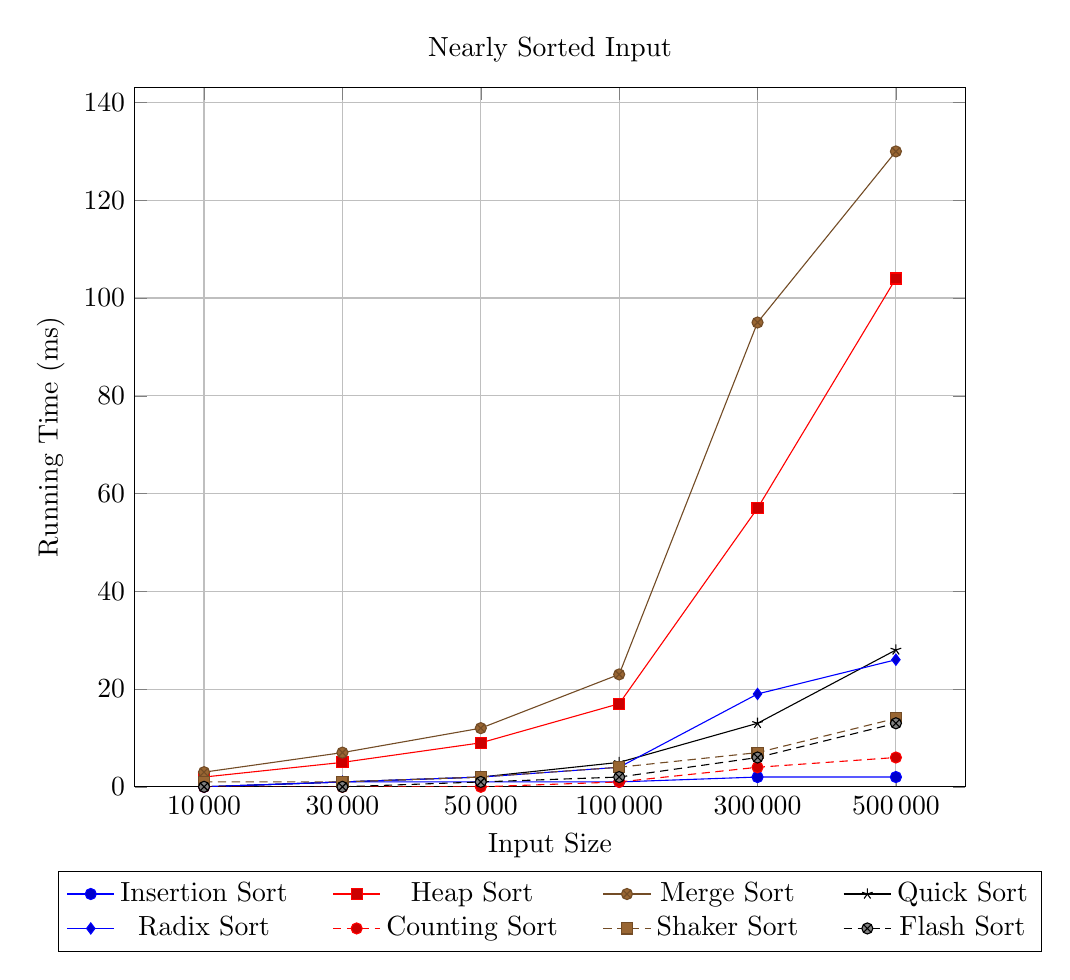
\begin{tikzpicture}
    \begin{axis}[
        width=\textwidth,
        title={Nearly Sorted Input},
        xlabel={Input Size},
        ylabel={Running Time (ms)},
        legend style={
            at={(0.5,-0.12)}, anchor=north, legend columns=4, 
            /tikz/every even column/.append style={column sep=0.5cm}
        },
        symbolic x coords={10\,000, 30\,000, 50\,000, 100\,000, 300\,000, 500\,000},
        xtick=data,
        ymin=0,
        grid=major,
    ]
    
    \addplot coordinates {(10\,000,0) (30\,000,1) (50\,000,1) 
    (100\,000,1) (300\,000,2) (500\,000,2)};
    \addlegendentry{Insertion Sort}
    
    \addplot coordinates {(10\,000,2) (30\,000,5) (50\,000,9) 
    (100\,000,17) (300\,000,57) (500\,000,104)};
    \addlegendentry{Heap Sort}
    
    \addplot coordinates {(10\,000,3) (30\,000,7) (50\,000,12) 
    (100\,000,23) (300\,000,95) (500\,000,130)};
    \addlegendentry{Merge Sort}
    
    \addplot coordinates {(10\,000,0) (30\,000,1) (50\,000,2) 
    (100\,000,5) (300\,000,13) (500\,000,28)};
    \addlegendentry{Quick Sort}
    
    \addplot coordinates {(10\,000,0) (30\,000,1) (50\,000,2) 
    (100\,000,4) (300\,000,19) (500\,000,26)};
    \addlegendentry{Radix Sort}
    
    \addplot coordinates {(10\,000,0) (30\,000,0) (50\,000,0) 
    (100\,000,1) (300\,000,4) (500\,000,6)};
    \addlegendentry{Counting Sort}
    
    \addplot coordinates {(10\,000,1) (30\,000,1) (50\,000,2) 
    (100\,000,4) (300\,000,7) (500\,000,14)};
    \addlegendentry{Shaker Sort}
    
    \addplot coordinates {(10\,000,0) (30\,000,0) (50\,000,1) 
    (100\,000,2) (300\,000,6) (500\,000,13)};
    \addlegendentry{Flash Sort}
    
    \end{axis}
\end{tikzpicture}
\caption{Kết quả thực nghiệm với đầu vào có thứ tự gần được sắp xếp (Nhóm 2)}
\end{figure}

\begin{itemize}[label=$\circ$]
    \item Các thuật toán như Selection Sort, Shell Sort, Bubble Sort, 
    Merge Sort và Heap Sort đều không có nhiều cải thiện. Ngược lại, 
    Shaker Sort, Insertion Sort và Quick Sort đã giảm đáng kể thời gian 
    thực thi xuống ngang bằng với nhóm thuật toán có độ phức tạp thời 
    gian là $O\left(n\right)$, thậm chí Insertion Sort còn giữ vị trí 
    nhanh nhất do chỉ cần đưa một vài phần tử nằm sai vị trí về đúng chỗ.
\end{itemize}

$\bullet$ Với đầu vào có thứ tự đã được sắp xếp \\

\begin{figure}[H]
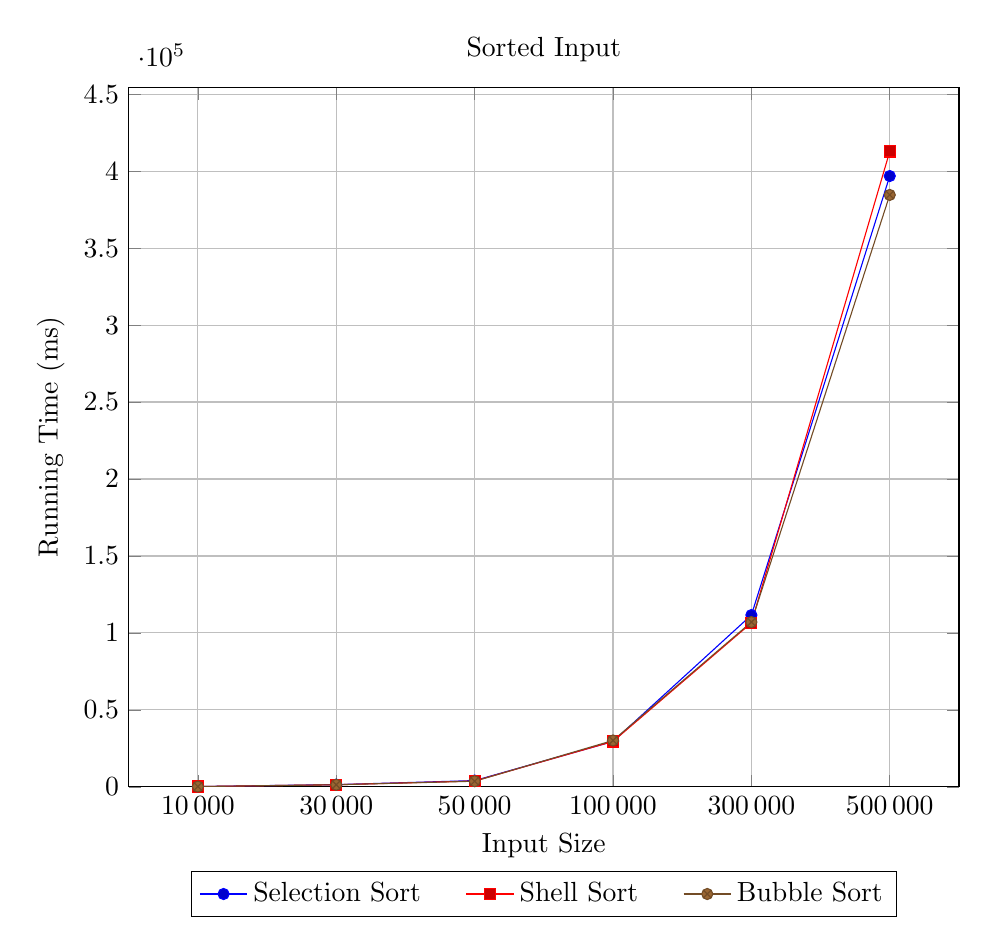
\begin{tikzpicture}
    \begin{axis}[
        width=\textwidth,
        title={Sorted Input},
        xlabel={Input Size},
        ylabel={Running Time (ms)},
        legend style={
            at={(0.5,-0.12)}, anchor=north, legend columns=3, 
            /tikz/every even column/.append style={column sep=0.5cm}
        },
        symbolic x coords={10\,000, 30\,000, 50\,000, 100\,000, 300\,000, 500\,000},
        xtick=data,
        ymin=0,
        grid=major,
    ]

    \addplot coordinates {(10\,000,182) (30\,000,1426) (50\,000,4059) 
    (100\,000,29478) (300\,000,111585) (500\,000,396841)};
    \addlegendentry{Selection Sort}
    
    \addplot coordinates {(10\,000,179) (30\,000,1349) (50\,000,3786) 
    (100\,000,29503) (300\,000,106498) (500\,000,412844)};
    \addlegendentry{Shell Sort}
    
    \addplot coordinates {(10\,000,180) (30\,000,1346) (50\,000,3636) 
    (100\,000,30120) (300\,000,107040) (500\,000,384574)};
    \addlegendentry{Bubble Sort}
    \end{axis}
\end{tikzpicture}
\caption{Kết quả thực nghiệm với đầu vào có thứ tự đã được sắp xếp (Nhóm 1)}
\end{figure}

\begin{figure}[H]
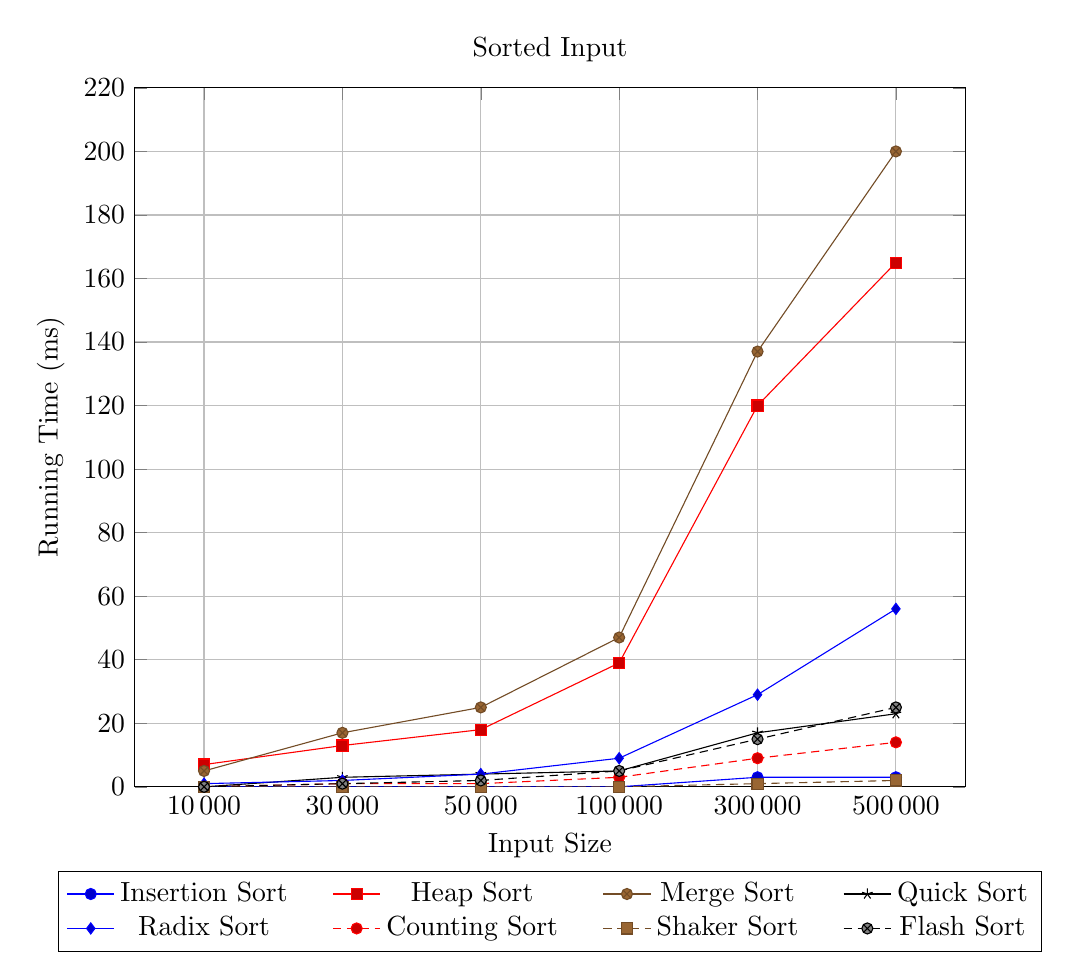
\begin{tikzpicture}
    \begin{axis}[
        width=\textwidth,
        title={Sorted Input},
        xlabel={Input Size},
        ylabel={Running Time (ms)},
        legend style={
            at={(0.5,-0.12)}, anchor=north, legend columns=4, 
            /tikz/every even column/.append style={column sep=0.5cm}
        },
        symbolic x coords={10\,000, 30\,000, 50\,000, 100\,000, 300\,000, 500\,000},
        xtick=data,
        ymin=0,
        grid=major,
    ]
    
    \addplot coordinates {(10\,000,0) (30\,000,0) (50\,000,0) 
    (100\,000,0) (300\,000,3) (500\,000,3)};
    \addlegendentry{Insertion Sort}
    
    \addplot coordinates {(10\,000,7) (30\,000,13) (50\,000,18) 
    (100\,000,39) (300\,000,120) (500\,000,165)};
    \addlegendentry{Heap Sort}
    
    \addplot coordinates {(10\,000,5) (30\,000,17) (50\,000,25) 
    (100\,000,47) (300\,000,137) (500\,000,200)};
    \addlegendentry{Merge Sort}
    
    \addplot coordinates {(10\,000,0) (30\,000,3) (50\,000,4) 
    (100\,000,5) (300\,000,17) (500\,000,23)};
    \addlegendentry{Quick Sort}
    
    \addplot coordinates {(10\,000,1) (30\,000,2) (50\,000,4) 
    (100\,000,9) (300\,000,29) (500\,000,56)};
    \addlegendentry{Radix Sort}
    
    \addplot coordinates {(10\,000,0) (30\,000,1) (50\,000,1) 
    (100\,000,3) (300\,000,9) (500\,000,14)};
    \addlegendentry{Counting Sort}
    
    \addplot coordinates {(10\,000,0) (30\,000,0) (50\,000,0) 
    (100\,000,0) (300\,000,1) (500\,000,2)};
    \addlegendentry{Shaker Sort}
    
    \addplot coordinates {(10\,000,0) (30\,000,1) (50\,000,2) 
    (100\,000,5) (300\,000,15) (500\,000,25)};
    \addlegendentry{Flash Sort}
    
    \end{axis}
\end{tikzpicture}
\caption{Kết quả thực nghiệm với đầu vào có thứ tự đã được sắp xếp (Nhóm 2)}
\end{figure}

\begin{itemize}
    \item Trong nhóm thuật toán có độ phức tạp $O\left(n^2\right)$ thì 
    Insertion Sort và Shaker Sort có tốc độ rất nhanh và hầu như là không 
    tốn thời gian với 100,000 phần tử. Ngược lại, 2 thuật toán còn lại 
    là Select Sort và Bubble Sort thì lại tốn khá nhiều thời gian và có 
    thời gian chạy không chênh lệch nhiều so với nhau.
    \item Trong nhóm thuật toán có độ phức tạp $O\left(n\log{n}\right)$ 
    thì Shell Sort lại dường như tốn rất nhiều thời gian tương đương với 
    một số thuật toán thuộc $O\left(n^2\right)$, còn Quick Sort là thuật 
    toán có thời gian chạy nhanh nhất, Heap Sort thì nhanh hơn Merge Sort 
    một chút.
    \item Trong nhóm thuật toán có độ phức tạp $O\left(n\right)$ thì 
    Counting Sort vẫn có thời gian chạy nhanh nhất, còn Radix Sort thì 
    có thời gian chạy chậm nhất trong nhóm thuật toán này.
\end{itemize}

$\bullet$ Với đầu vào có thứ tự được sắp xếp ngược \\

\begin{figure}[H]
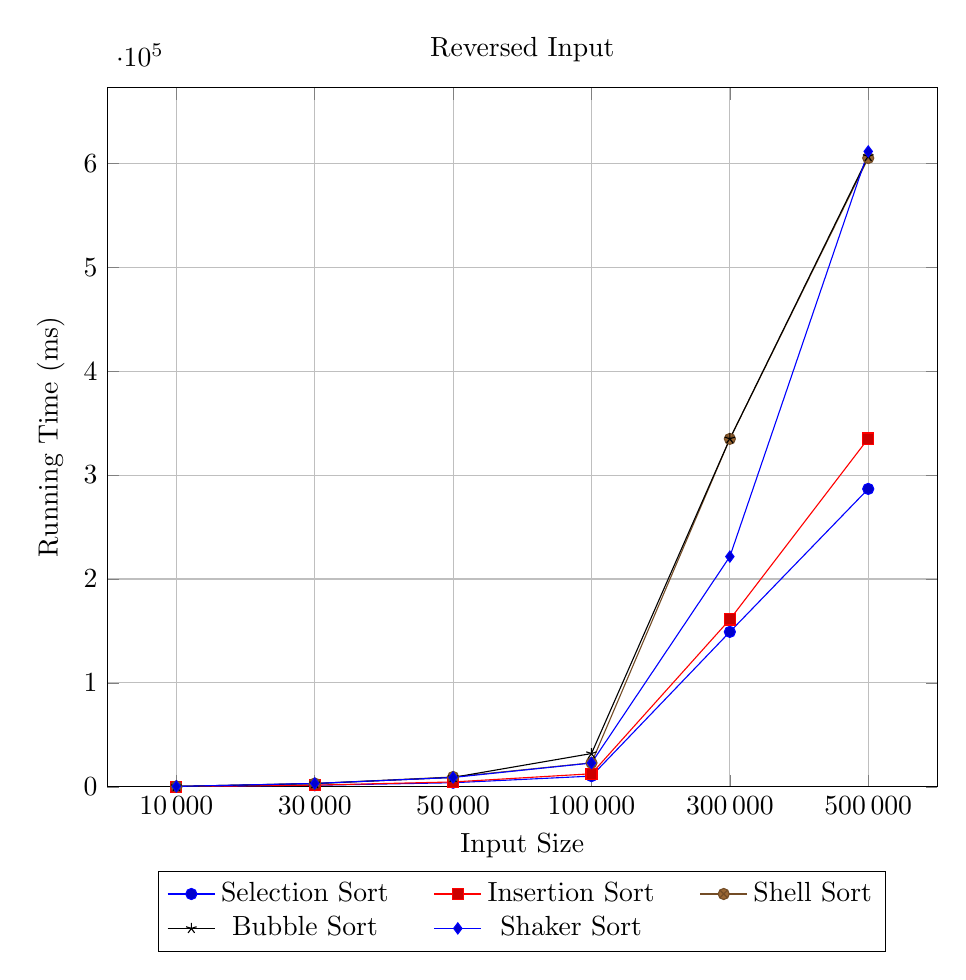
\begin{tikzpicture}
    \begin{axis}[
        width=\textwidth,
        title={Reversed Input},
        xlabel={Input Size},
        ylabel={Running Time (ms)},
        legend style={
            at={(0.5,-0.12)}, anchor=north, legend columns=3, 
            /tikz/every even column/.append style={column sep=0.5cm}
        },
        symbolic x coords={10\,000, 30\,000, 50\,000, 100\,000, 300\,000, 500\,000},
        xtick=data,
        ymin=0,
        grid=major,
    ]
    
    \addplot coordinates {(10\,000,175) (30\,000,1477) (50\,000,3924) 
    (100\,000,10289) (300\,000,149091) (500\,000,286666)};
    \addlegendentry{Selection Sort}
    
    \addplot coordinates {(10\,000,202) (30\,000,1630) (50\,000,4686) 
    (100\,000,12560) (300\,000,161038) (500\,000,335113)};
    \addlegendentry{Insertion Sort}
    
    \addplot coordinates {(10\,000,383) (30\,000,3158) (50\,000,9485) 
    (100\,000,23060) (300\,000,334815) (500\,000,605040)};
    \addlegendentry{Shell Sort}
    
    \addplot coordinates {(10\,000,373) (30\,000,3116) (50\,000,9043) 
    (100\,000,32013) (300\,000,334914) (500\,000,606656)};
    \addlegendentry{Bubble Sort}
    
    \addplot coordinates {(10\,000,385) (30\,000,3255) (50\,000,9005) 
    (100\,000,22892) (300\,000,221549) (500\,000,611441)};
    \addlegendentry{Shaker Sort}
    
    \end{axis}
\end{tikzpicture}
\caption{Kết quả thực nghiệm với đầu vào có thứ tự được sắp xếp ngược (Nhóm 1)}
\end{figure}

\begin{figure}[H]
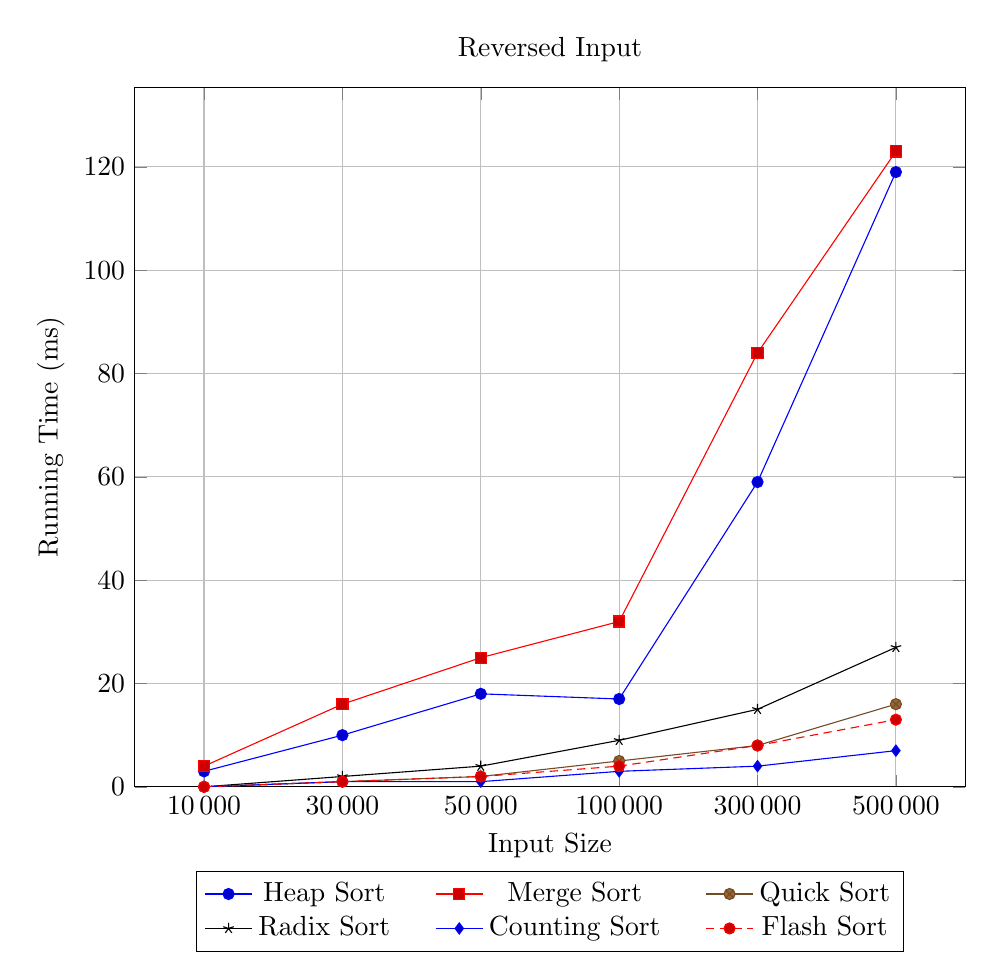
\begin{tikzpicture}
    \begin{axis}[
        width=\textwidth,
        title={Reversed Input},
        xlabel={Input Size},
        ylabel={Running Time (ms)},
        legend style={
            at={(0.5,-0.12)}, anchor=north, legend columns=3, 
            /tikz/every even column/.append style={column sep=0.5cm}
        },
        symbolic x coords={10\,000, 30\,000, 50\,000, 100\,000, 300\,000, 500\,000},
        xtick=data,
        ymin=0,
        grid=major,
    ]
    
    \addplot coordinates {(10\,000,3) (30\,000,10) (50\,000,18) 
    (100\,000,17) (300\,000,59) (500\,000,119)};
    \addlegendentry{Heap Sort}
    
    \addplot coordinates {(10\,000,4) (30\,000,16) (50\,000,25) 
    (100\,000,32) (300\,000,84) (500\,000,123)};
    \addlegendentry{Merge Sort}
    
    \addplot coordinates {(10\,000,0) (30\,000,1) (50\,000,2) 
    (100\,000,5) (300\,000,8) (500\,000,16)};
    \addlegendentry{Quick Sort}
    
    \addplot coordinates {(10\,000,0) (30\,000,2) (50\,000,4) 
    (100\,000,9) (300\,000,15) (500\,000,27)};
    \addlegendentry{Radix Sort}
    
    \addplot coordinates {(10\,000,0) (30\,000,1) (50\,000,1) 
    (100\,000,3) (300\,000,4) (500\,000,7)};
    \addlegendentry{Counting Sort}
    
    \addplot coordinates {(10\,000,0) (30\,000,1) (50\,000,2) 
    (100\,000,4) (300\,000,8) (500\,000,13)};
    \addlegendentry{Flash Sort}
    
    \end{axis}
\end{tikzpicture}
\caption{Kết quả thực nghiệm với đầu vào có thứ tự được sắp xếp ngược (Nhóm 2)}
\end{figure}

\begin{itemize}[label=$\circ$]
    \item Các thuật toán như Selection Sort, Shell Sort, Bubble Sort, 
    Merge Sort, và Heap Sort đều thể hiện thời gian thực thi cao, đặc 
    biệt là nhóm các thuật toán có độ phức tạp thời gian trung bình là 
    $O\left(n^2\right)$. Những thuật toán như Bubble Sort và Shaker Sort 
    trở nên chậm đáng kể do cần nhiều phép hoán đổi, trong khi Selection 
    Sort duy trì hiệu suất ổn định nhưng vẫn kém hiệu quả vì phải duyệt 
    toàn bộ danh sách để tìm giá trị nhỏ nhất.
    \item Ngược lại, nhóm thuật toán có độ phức tạp trung bình là 
    $O\left(n\log{n}\right)$ như Quick Sort, Merge Sort và Heap Sort thể 
    hiện hiệu suất vượt trội hơn, với Merge Sort và Heap Sort ổn định hơn 
    so với Quick Sort do đặc thù phân chia dữ liệu của chúng.
    \item Đặc biệt, các thuật toán có độ phức tạp $O\left(n\right)$ như 
    Counting Sort và Flash Sort cho thấy thời gian thực thi thấp nhất 
    trong các biểu đồ, chứng minh tính vượt trội khi xử lý các dữ liệu 
    lớn ngay cả trong trường hợp xấu nhất.
\end{itemize}

\subsubsection{Về số phép so sánh}

$\bullet$ Với đầu vào có thứ tự ngẫu nhiên \\

\begin{figure}[H]
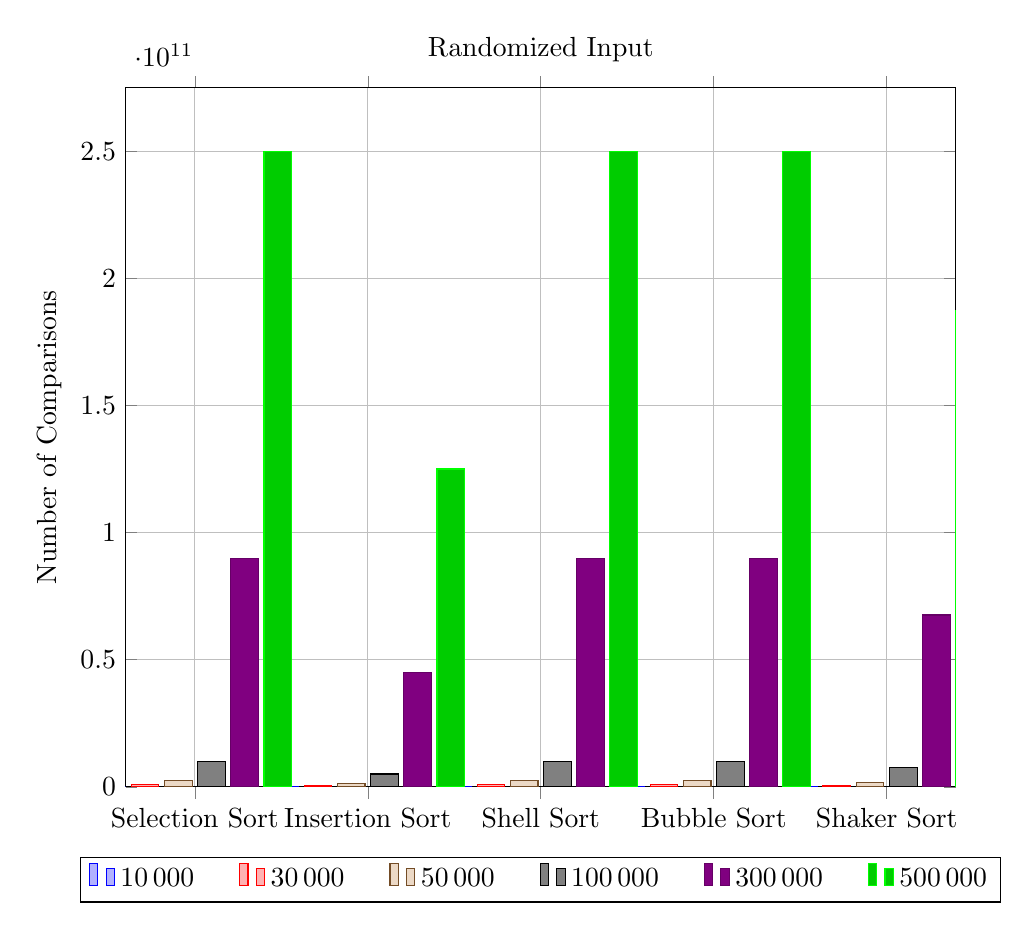
\begin{tikzpicture}
    \begin{axis}[
        width=\textwidth,
        title={Randomized Input},
        ybar,
        ymin=0,
        grid=major,
        legend style={
            at={(0.5,-0.1)}, anchor=north, legend columns=-1,
            /tikz/every even column/.append style={column sep=0.5cm}
        },
        ylabel={Number of Comparisons},
        symbolic x coords={
            Selection Sort, Insertion Sort, Shell Sort, Bubble Sort, 
            Shaker Sort
        },
        xtick=data,
    ]
    \addplot coordinates {(Selection Sort,100009999) 
        (Insertion Sort,49852722) (Shell Sort,100009999) 
        (Bubble Sort,100009999) (Shaker Sort,75877345)};
    \addplot coordinates {(Selection Sort,900029999) 
        (Insertion Sort,450424387) (Shell Sort,900029999) 
        (Bubble Sort,900029999) (Shaker Sort,678034901)};
    \addplot coordinates {(Selection Sort,2500049999) 
        (Insertion Sort,1244875082) (Shell Sort,2500049999) 
        (Bubble Sort,2500049999) (Shaker Sort,1868558231)};
    \addplot coordinates {(Selection Sort,10000099999) 
        (Insertion Sort,5026592949) (Shell Sort,10000099999) 
        (Bubble Sort,10000099999) (Shaker Sort,7519014091)};
    \addplot coordinates {(Selection Sort,90000299999) 
        (Insertion Sort,44937080911) (Shell Sort,90000299999) 
        (Bubble Sort,90000299999) (Shaker Sort,67598742089)};
    \addplot coordinates {(Selection Sort,250000499999) 
        (Insertion Sort,125044404674) (Shell Sort,250000499999) 
        (Bubble Sort,250000499999) (Shaker Sort,187569730819)};
        \legend{10\,000, 30\,000, 50\,000, 100\,000, 300\,000, 500\,000}
    \end{axis}
\end{tikzpicture}
\caption{Kết quả thực nghiệm với đầu vào có thứ tự ngẫu nhiên (Nhóm 1)}
\end{figure}

\begin{figure}[H]
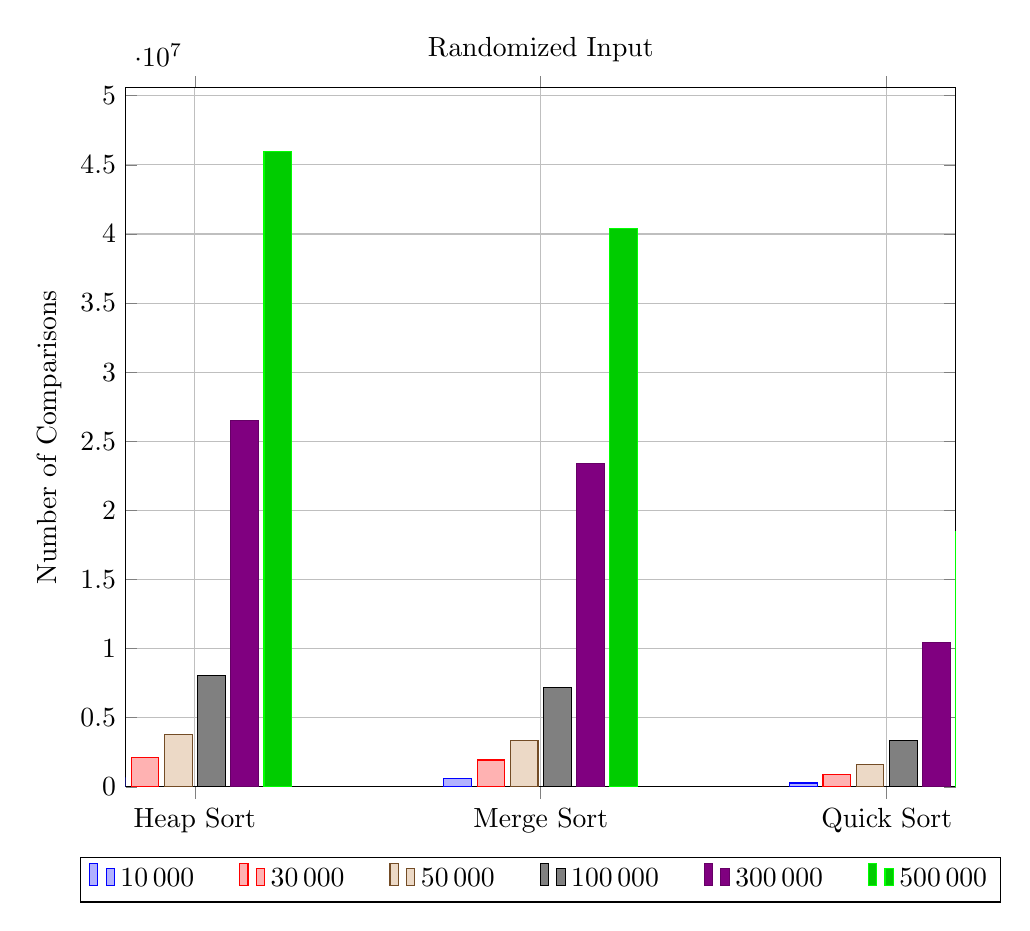
\begin{tikzpicture}
    \begin{axis}[
        width=\textwidth,
        title={Randomized Input},
        ybar,
        ymin=0,
        grid=major,
        legend style={
            at={(0.5,-0.1)}, anchor=north, legend columns=-1,
            /tikz/every even column/.append style={column sep=0.5cm}
        },
        ylabel={Number of Comparisons},
        symbolic x coords={Heap Sort, Merge Sort, Quick Sort},
        xtick=data,
    ]
    \addplot coordinates {(Heap Sort,638425) 
        (Merge Sort,583832) (Quick Sort,276045)};
    \addplot coordinates {(Heap Sort,2150786) 
        (Merge Sort,1937240) (Quick Sort,916849)};
    \addplot coordinates {(Heap Sort,3771772) 
        (Merge Sort,3383319) (Quick Sort,1636700)};
    \addplot coordinates {(Heap Sort,8044992) 
        (Merge Sort,7166010) (Quick Sort,3341712)};
    \addplot coordinates {(Heap Sort,26487787) 
        (Merge Sort,23383601) (Quick Sort,10434674)};
    \addplot coordinates {(Heap Sort,45972193) 
        (Merge Sort,40383061) (Quick Sort,18476753)};
    \legend{10\,000, 30\,000, 50\,000, 100\,000, 300\,000, 500\,000}
    \end{axis}
\end{tikzpicture}
\caption{Kết quả thực nghiệm với đầu vào có thứ tự ngẫu nhiên (Nhóm 2)}
\end{figure}

\begin{figure}[H]
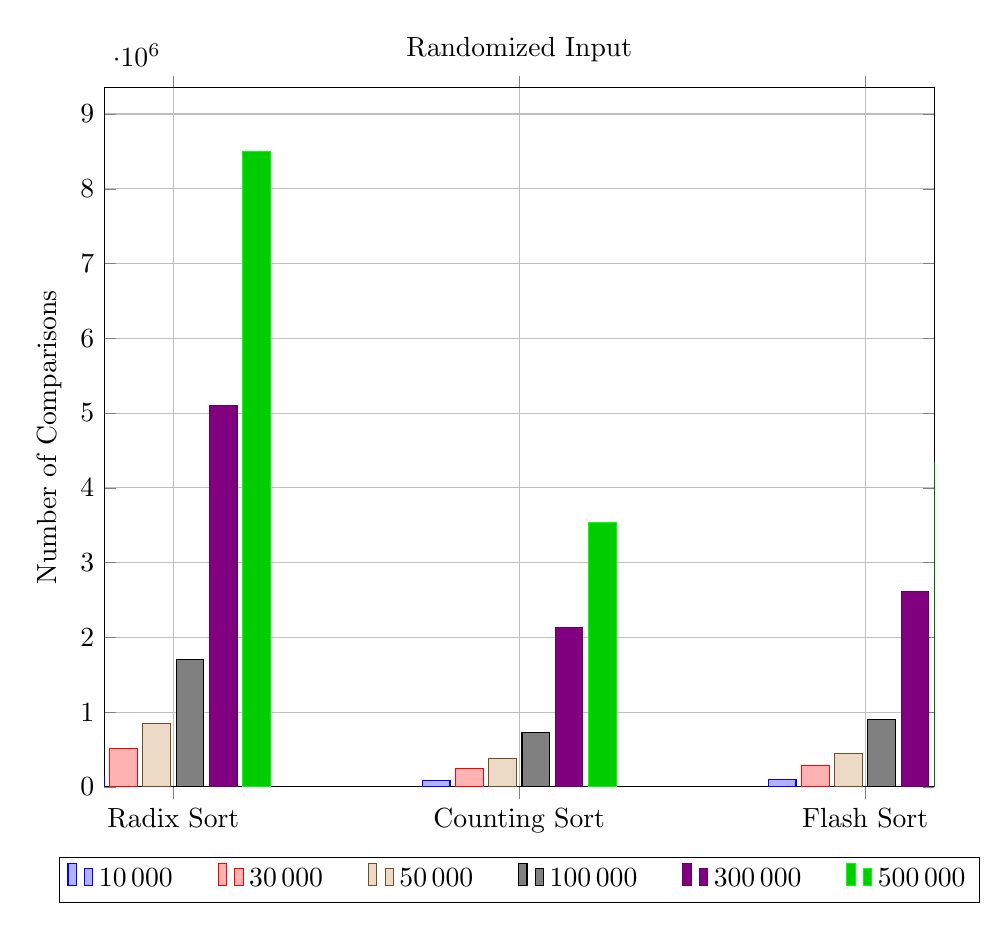
\begin{tikzpicture}
    \begin{axis}[
        width=\textwidth,
        title={Randomized Input},
        ybar,
        ymin=0,
        grid=major,
        legend style={
            at={(0.5,-0.1)}, anchor=north, legend columns=-1,
            /tikz/every even column/.append style={column sep=0.5cm}
        },
        ylabel={Number of Comparisons},
        symbolic x coords={Radix Sort, Counting Sort, Flash Sort},
        xtick=data,
    ]
    \addplot coordinates {(Radix Sort,140056) 
        (Counting Sort,80000) (Flash Sort,97658)};
    \addplot coordinates {(Radix Sort,510070) 
        (Counting Sort,240000) (Flash Sort,285201)};
    \addplot coordinates {(Radix Sort,850070) 
        (Counting Sort,382769) (Flash Sort,451390)};
    \addplot coordinates {(Radix Sort,1700070) 
        (Counting Sort,732769) (Flash Sort,905677)};
    \addplot coordinates {(Radix Sort,5100070) 
        (Counting Sort,2132769) (Flash Sort,2611012)};
    \addplot coordinates {(Radix Sort,8500070) 
        (Counting Sort,3532769) (Flash Sort,4335083)};
    \legend{10\,000, 30\,000, 50\,000, 100\,000, 300\,000, 500\,000}
    \end{axis}
\end{tikzpicture}
\caption{Kết quả thực nghiệm với đầu vào có thứ tự ngẫu nhiên (Nhóm 3)}
\end{figure}

\begin{itemize}[label=$\circ$]
    \item Có thể nhận xét rằng số phép so sánh giữa các thuật toán sắp 
    xếp thay đổi đáng kể tùy thuộc vào độ phức tạp về thời gian của từng 
    thuật toán. Nhóm các thuật toán có số phép so sánh lớn nhất bao gồm 
    Selection Sort, Insertion Sort, Shell Sort, Bubble Sort và Shaker 
    Sort do có độ phức tạp $O\left(n^2\right)$. Trong đó, cả 3 thuật toán 
    gồm Selection Sort, Shell Sort, Bubble Sort đều có số phép so sánh 
    bằng nhau và lớn nhất so với 8 thuật toán còn lại. Điều này dẫn đến 
    số phép so sánh tăng nhanh khi kích thước mảng lớn, đặc biệt là ở các 
    mảng kích thước 300000 và 500000, với cột biểu đồ vượt trội hơn hẳn 
    so với các thuật toán khác.
	\item Trong khi đó, nhóm thuật toán có hiệu suất trung bình như Heap 
    Sort, Merge Sort, và Quick Sort hoạt động hiệu quả hơn nhờ độ phức 
    tạp $O\left(n\log{n}\right)$. Quick Sort có số phép so sánh thấp hơn 
    so với Heap Sort và Merge Sort, cho thấy ưu thế rõ rệt khi xử lý trên 
    mảng ngẫu nhiên.
	\item Cuối cùng, nhóm thuật toán có số phép so sánh thấp nhất bao 
    gồm Radix Sort, Counting Sort, và Flash Sort, nhờ đặc điểm không dựa 
    trên các phép so sánh với độ phức tạp gần như là $O\left(n\right)$. 
    Counting Sort đặc biệt nổi bật với số phép so sánh thấp nhất trong 
    nhóm này và thấp nhất trong 11 thuật toán.
\end{itemize}

$\bullet$ Với đầu vào có thứ tự gần được sắp xếp \\

\begin{figure}[H]
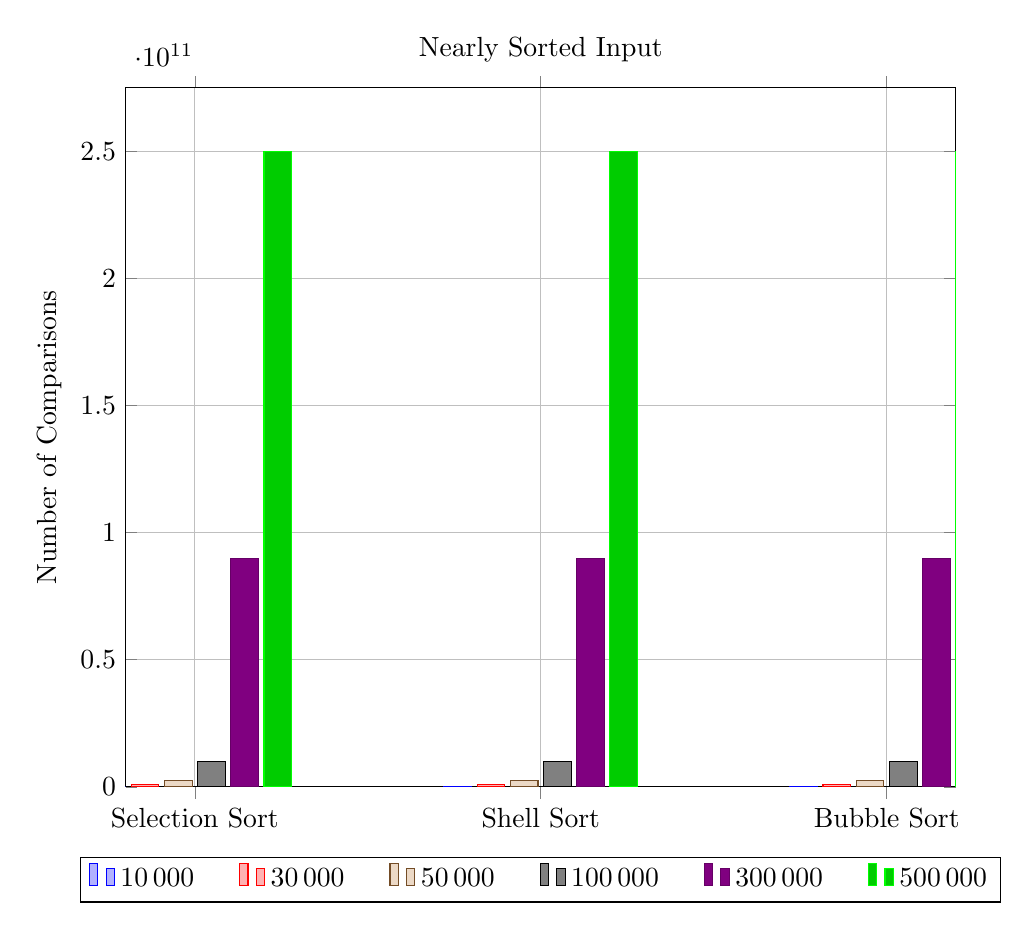
\begin{tikzpicture}
    \begin{axis}[
        width=\textwidth,
        title={Nearly Sorted Input},
        ybar,
        ymin=0,
        grid=major,
        legend style={
            at={(0.5,-0.1)}, anchor=north, legend columns=-1,
            /tikz/every even column/.append style={column sep=0.5cm}
        },
        ylabel={Number of Comparisons},
        symbolic x coords={Selection Sort, Shell Sort, Bubble Sort},
        xtick=data,
    ]
    \addplot coordinates {(Selection Sort,100009999) 
        (Shell Sort,100009999) (Bubble Sort,100009999)};
    \addplot coordinates {(Selection Sort,900029999) 
        (Shell Sort,900029999) (Bubble Sort,900029999)};
    \addplot coordinates {(Selection Sort,2500049999) 
        (Shell Sort,2500049999) (Bubble Sort,2500049999)};
    \addplot coordinates {(Selection Sort,10000099999) 
        (Shell Sort,10000099999) (Bubble Sort,10000099999)};
    \addplot coordinates {(Selection Sort,90000299999) 
        (Shell Sort,90000299999) (Bubble Sort,90000299999)};
    \addplot coordinates {(Selection Sort,250000499999) 
        (Shell Sort,250000499999) (Bubble Sort,250000499999)};
    \legend{10\,000, 30\,000, 50\,000, 100\,000, 300\,000, 500\,000}
    \end{axis}
\end{tikzpicture}
\caption{Kết quả thực nghiệm với đầu vào có thứ tự gần được sắp xếp (Nhóm 1)}
\end{figure}

\begin{figure}[H]
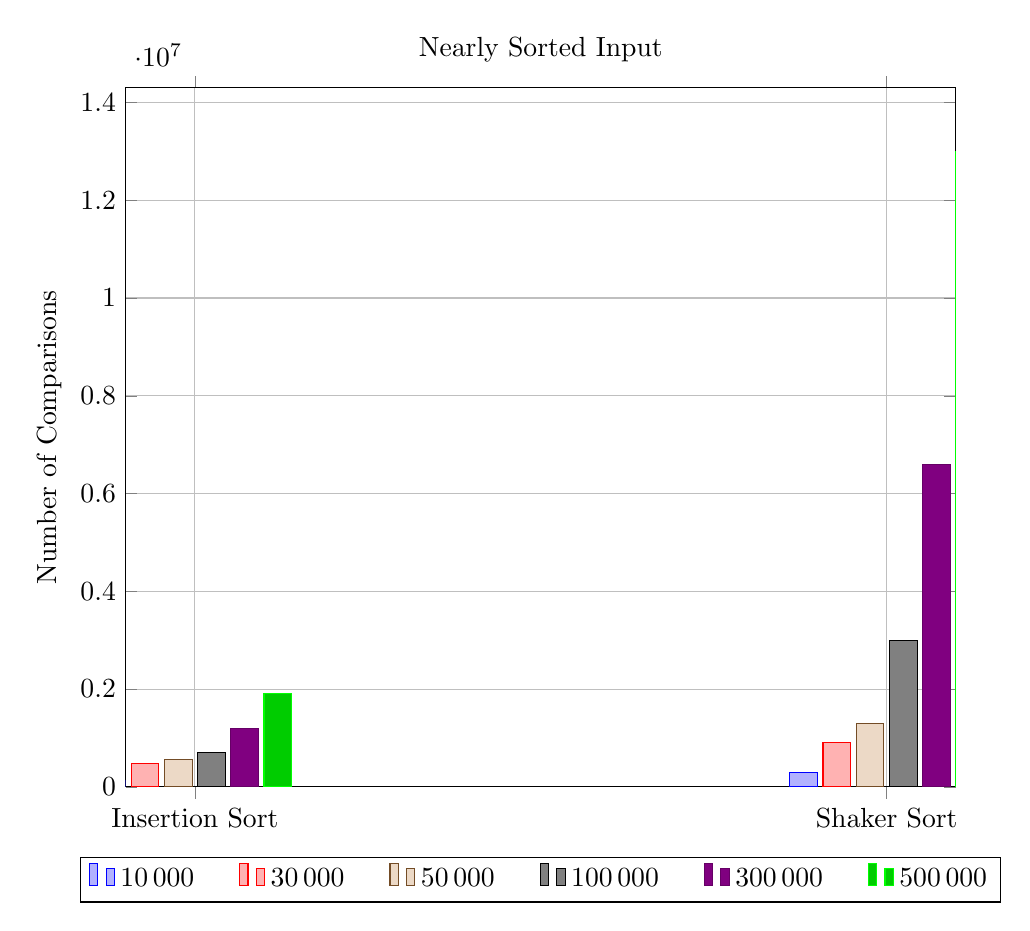
\begin{tikzpicture}
    \begin{axis}[
        width=\textwidth,
        title={Nearly Sorted Input},
        ybar,
        ymin=0,
        grid=major,
        legend style={
            at={(0.5,-0.1)}, anchor=north, legend columns=-1,
            /tikz/every even column/.append style={column sep=0.5cm}
        },
        ylabel={Number of Comparisons},
        symbolic x coords={Insertion Sort, Shaker Sort},
        xtick=data,
    ]
    \addplot coordinates {(Insertion Sort,129726) 
        (Shaker Sort,299791)};
    \addplot coordinates {(Insertion Sort,486366) 
        (Shaker Sort,899791)};
    \addplot coordinates {(Insertion Sort,560354) 
        (Shaker Sort,1299845)};
    \addplot coordinates {(Insertion Sort,706102) 
        (Shaker Sort,2999791)};
    \addplot coordinates {(Insertion Sort,1188582) 
        (Shaker Sort,6599891)};
    \addplot coordinates {(Insertion Sort,1905186) 
        (Shaker Sort,12999845)};
    \legend{10\,000, 30\,000, 50\,000, 100\,000, 300\,000, 500\,000}
    \end{axis}
\end{tikzpicture}
\caption{Kết quả thực nghiệm với đầu vào có thứ tự gần được sắp xếp (Nhóm 2)}
\end{figure}

\begin{figure}[H]
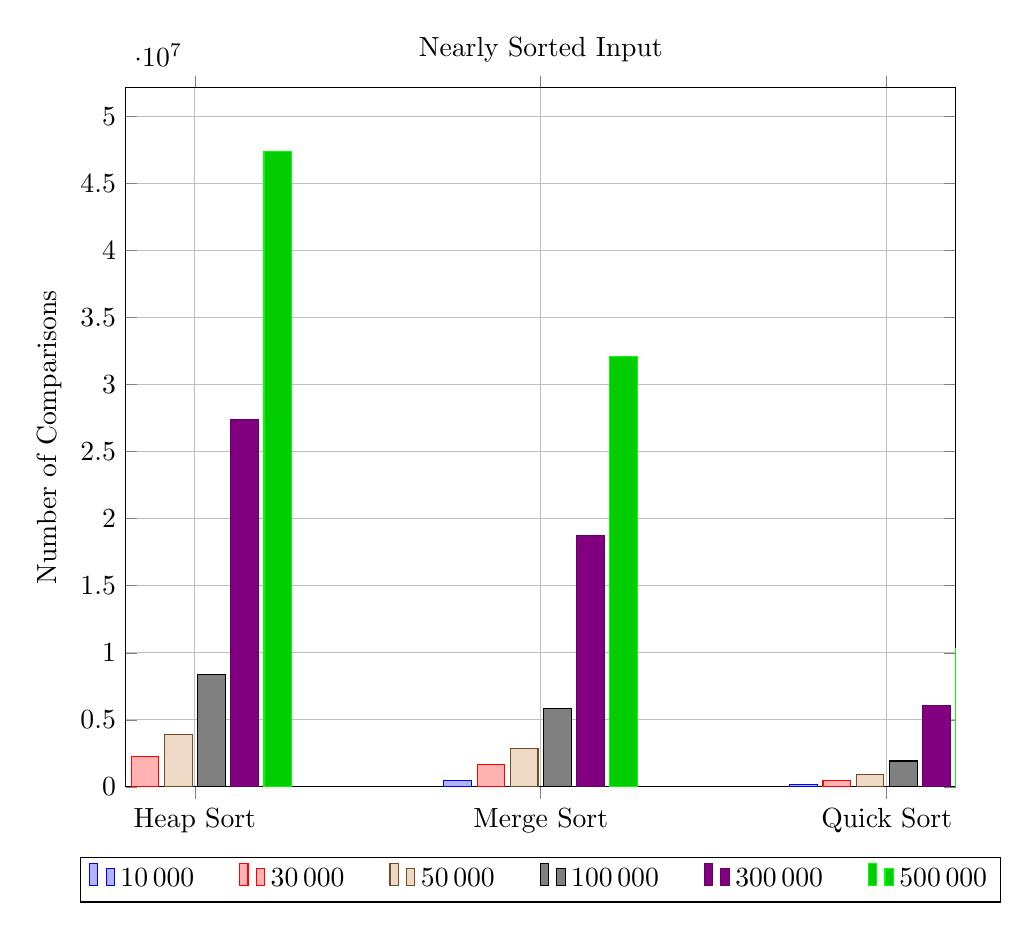
\begin{tikzpicture}
    \begin{axis}[
        width=\textwidth,
        title={Nearly Sorted Input},
        ybar,
        ymin=0,
        grid=major,
        legend style={
            at={(0.5,-0.1)}, anchor=north, legend columns=-1,
            /tikz/every even column/.append style={column sep=0.5cm}
        },
        ylabel={Number of Comparisons},
        symbolic x coords={Heap Sort, Merge Sort, Quick Sort},
        xtick=data,
    ]
    \addplot coordinates {(Heap Sort,669904) 
        (Merge Sort,503802) (Quick Sort,154995)};
    \addplot coordinates {(Heap Sort,2236774) 
        (Merge Sort,1637853) (Quick Sort,501973)};
    \addplot coordinates {(Heap Sort,3925280) 
        (Merge Sort,2845326) (Quick Sort,913890)};
    \addplot coordinates {(Heap Sort,8364715) 
        (Merge Sort,5851166) (Quick Sort,1927723)};
    \addplot coordinates {(Heap Sort,27413296) 
        (Merge Sort,18733795) (Quick Sort,6058264)};
    \addplot coordinates {(Heap Sort,47405047) 
        (Merge Sort,32137705) (Quick Sort,10310769)};
    \legend{10\,000, 30\,000, 50\,000, 100\,000, 300\,000, 500\,000}
    \end{axis}
\end{tikzpicture}
\caption{Kết quả thực nghiệm với đầu vào có thứ tự gần được sắp xếp (Nhóm 3)}
\end{figure}

\begin{figure}[H]
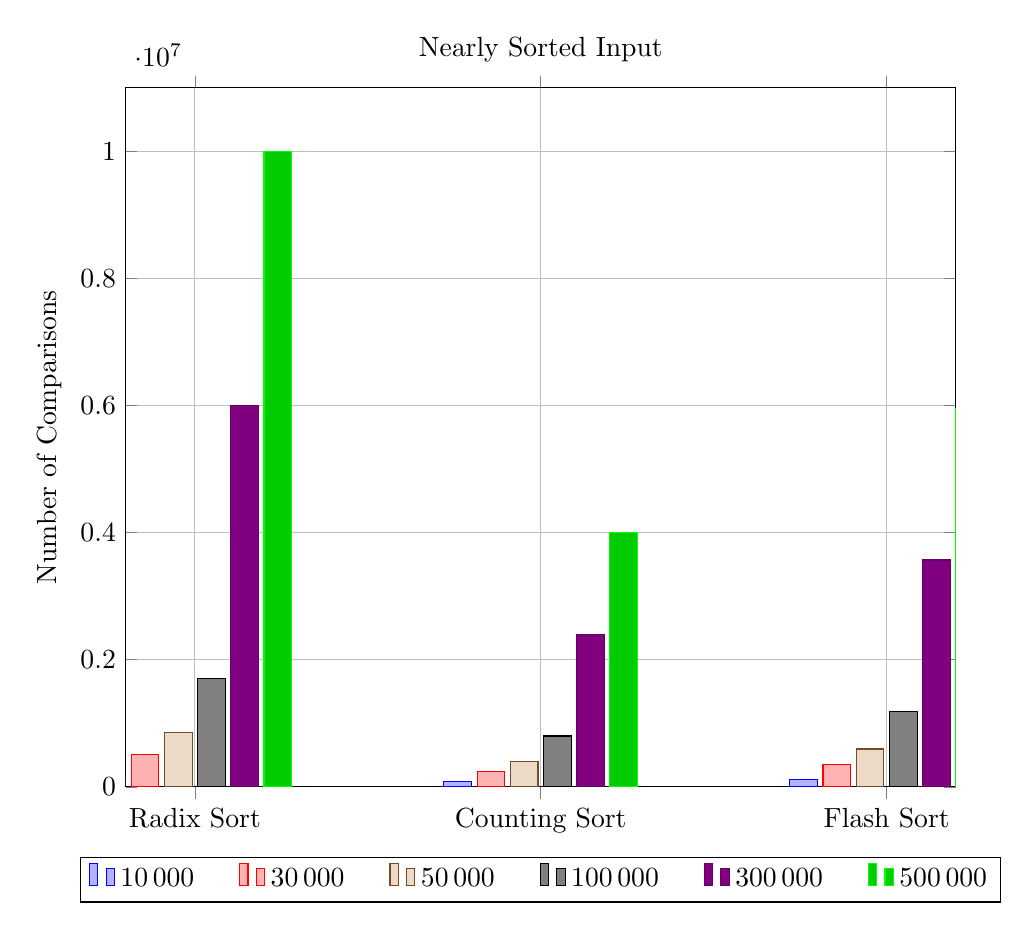
\begin{tikzpicture}
    \begin{axis}[
        width=\textwidth,
        title={Nearly Sorted Input},
        ybar,
        ymin=0,
        grid=major,
        legend style={
            at={(0.5,-0.1)}, anchor=north, legend columns=-1,
            /tikz/every even column/.append style={column sep=0.5cm}
        },
        ylabel={Number of Comparisons},
        symbolic x coords={Radix Sort, Counting Sort, Flash Sort},
        xtick=data,
    ]
    \addplot coordinates {(Radix Sort,140056) 
        (Counting Sort,80001) (Flash Sort,118969)};
    \addplot coordinates {(Radix Sort,510070) 
        (Counting Sort,240001) (Flash Sort,356969)};
    \addplot coordinates {(Radix Sort,850070) 
        (Counting Sort,400001) (Flash Sort,594969)};
    \addplot coordinates {(Radix Sort,1700070) 
        (Counting Sort,800001) (Flash Sort,1189967)};
    \addplot coordinates {(Radix Sort,6000084) 
        (Counting Sort,2400001) (Flash Sort,3569970)};
    \addplot coordinates {(Radix Sort,10000084) 
        (Counting Sort,4000001) (Flash Sort,5949970)};
    \legend{10\,000, 30\,000, 50\,000, 100\,000, 300\,000, 500\,000}
    \end{axis}
\end{tikzpicture}
\caption{Kết quả thực nghiệm với đầu vào có thứ tự gần được sắp xếp (Nhóm 4)}
\end{figure}

\begin{itemize}[label=$\circ$]
    \item Có thể nhận xét rằng số phép so sánh giữa các thuật toán sắp 
    xếp thay đổi đáng kể tùy thuộc vào độ phức tạp về thời gian và khả 
    năng tối ưu hóa đối với mảng đã có trật tự. Nhóm các thuật toán có 
    số phép so sánh lớn nhất bao gồm Selection Sort, Shell Sort, và 
    Bubble Sort do có độ phức tạp $O\left(n^2\right)$ và không tận dụng 
    được tính chất mảng gần như đã sắp xếp. Trong đó, cả ba thuật toán 
    này đều có số phép so sánh cao nhất, đặc biệt khi kích thước mảng 
    tăng lên 300000 và 500000, với cột biểu đồ vượt trội so với các 
    thuật toán khác. Insertion Sort, nhờ khả năng tối ưu hóa tốt cho 
    các mảng đã gần sắp xếp, thực hiện ít phép so sánh hơn đáng kể, 
    trong khi Shaker Sort (một biến thể của Bubble Sort) cũng cho thấy 
    hiệu năng cải thiện nhưng vẫn kém hiệu quả hơn Insertion Sort. 
	\item Đối với các thuật toán có độ phức tạp là $O\left(n\log{n}\right)$ 
    về thời gian, Heap Sort thực hiện nhiều phép so sánh hơn so với Merge 
    Sort và Quick Sort. Trong đó, Quick Sort tỏ ra vượt trội hơn Merge 
    Sort nhờ khả năng tận dụng tốt tính chất của mảng gần như được sắp xếp. 
	\item Cuối cùng, nhóm thuật toán có số phép so sánh thấp nhất bao 
    gồm Radix Sort, Counting Sort và Flash Sort, nhờ đặc điểm không phụ 
    thuộc vào số phép so sánh với độ phức tạp gần như là $O\left(n\right)$. 
    Nhóm này không chỉ có số phép so sánh thấp nhất mà còn duy trì hiệu 
    năng ổn định ngay cả khi kích thước mảng tăng cao. Đặc biệt, Counting 
    Sort có số phép so sánh nhỏ nhất với tất cả kích thước đầu vào trong 
    mảng có thứ tự gần được sắp xếp hoàn chỉnh.
\end{itemize}

$\bullet$ Với đầu vào có thứ tự đã được sắp xếp \\

\begin{figure}[H]
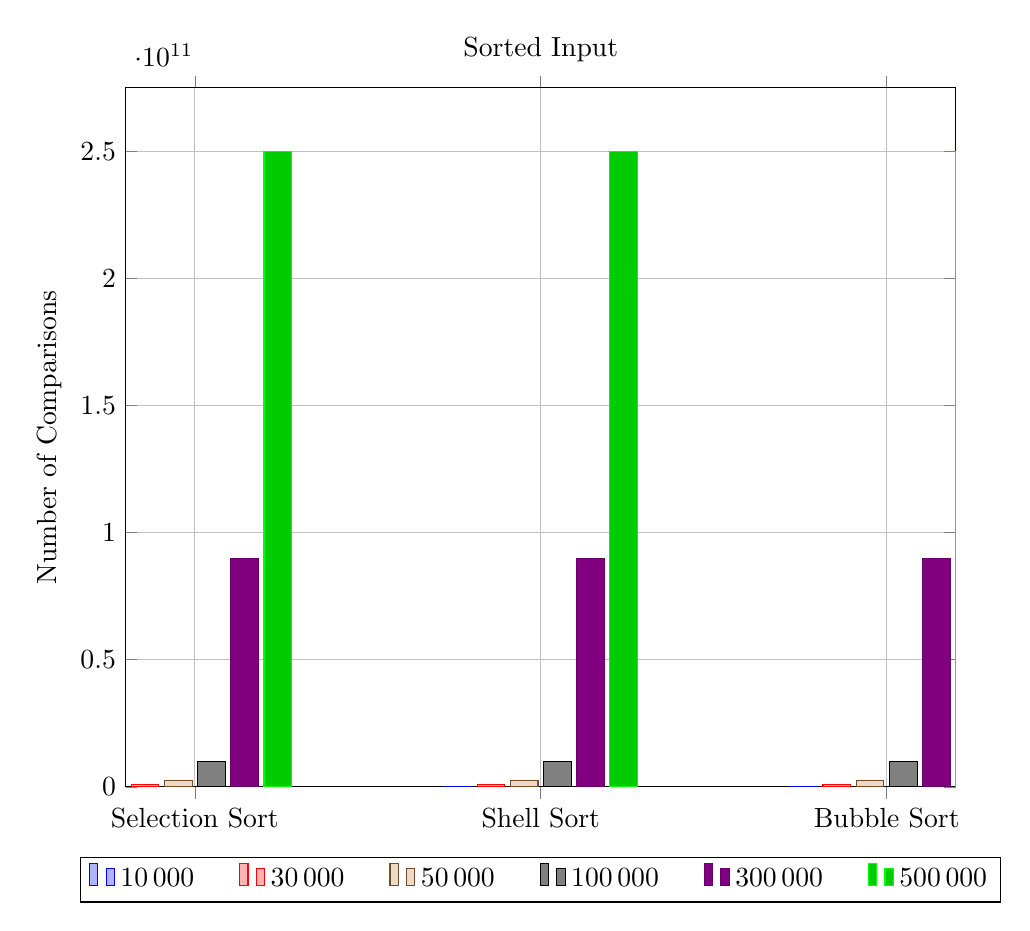
\begin{tikzpicture}
    \begin{axis}[
        width=\textwidth,
        title={Sorted Input},
        ybar,
        ymin=0,
        grid=major,
        legend style={
            at={(0.5,-0.1)}, anchor=north, legend columns=-1,
            /tikz/every even column/.append style={column sep=0.5cm}
        },
        ylabel={Number of Comparisons},
        symbolic x coords={Selection Sort, Shell Sort, Bubble Sort},
        xtick=data,
    ]
    \addplot coordinates {(Selection Sort,100009999) 
        (Shell Sort,100009999) (Bubble Sort,100009999)};
    \addplot coordinates {(Selection Sort,900029999) 
        (Shell Sort,900029999) (Bubble Sort,900029999)};
    \addplot coordinates {(Selection Sort,2500049999) 
        (Shell Sort,2500049999) (Bubble Sort,2500049999)};
    \addplot coordinates {(Selection Sort,10000099999) 
        (Shell Sort,10000099999) (Bubble Sort,10000099999)};
    \addplot coordinates {(Selection Sort,90000299999) 
        (Shell Sort,90000299999) (Bubble Sort,90000299999)};
    \addplot coordinates {(Selection Sort,250000499999) 
        (Shell Sort,250000499999) (Bubble Sort,250000499999)};
    \legend{10\,000, 30\,000, 50\,000, 100\,000, 300\,000, 500\,000}
    \end{axis}
\end{tikzpicture}
\caption{Kết quả thực nghiệm với đầu vào có thứ tự đã được sắp xếp (Nhóm 1)}
\end{figure}

\begin{figure}[H]
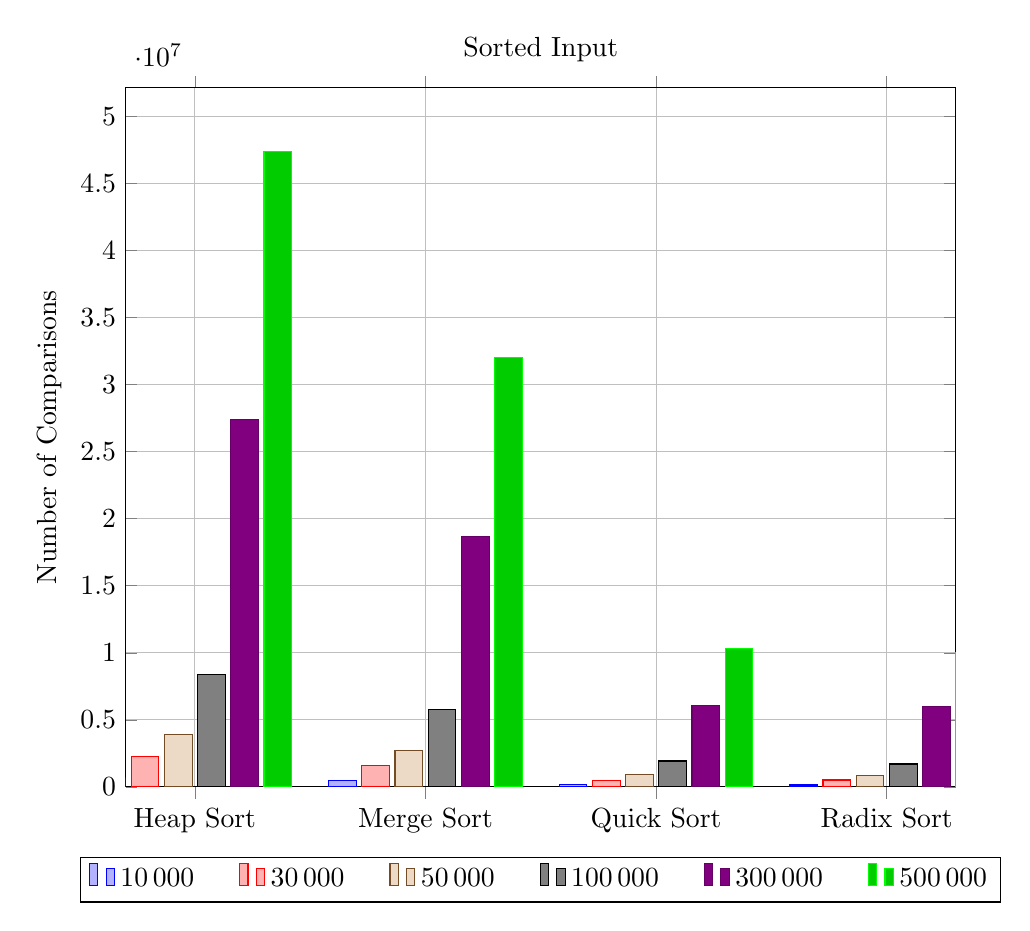
\begin{tikzpicture}
    \begin{axis}[
        width=\textwidth,
        title={Sorted Input},
        ybar,
        ymin=0,
        grid=major,
        legend style={
            at={(0.5,-0.1)}, anchor=north, legend columns=-1,
            /tikz/every even column/.append style={column sep=0.5cm}
        },
        ylabel={Number of Comparisons},
        symbolic x coords={Heap Sort, Merge Sort, Quick Sort, Radix Sort},
        xtick=data,
    ]
    \addplot coordinates {(Heap Sort,670329) (Merge Sort,475242) 
        (Quick Sort,154959) (Radix Sort,140056)};
    \addplot coordinates {(Heap Sort,2236648) (Merge Sort,1559914) 
        (Quick Sort,501929) (Radix Sort,510070)};
    \addplot coordinates {(Heap Sort,3925351) (Merge Sort,2722826) 
        (Quick Sort,913850) (Radix Sort,850070)};
    \addplot coordinates {(Heap Sort,8365080) (Merge Sort,5745658) 
        (Quick Sort,1927691) (Radix Sort,1700070)};
    \addplot coordinates {(Heap Sort,27413230) (Merge Sort,18645946) 
        (Quick Sort,6058228) (Radix Sort,6000084)};
    \addplot coordinates {(Heap Sort,47404886) (Merge Sort,32017850) 
        (Quick Sort,10310733) (Radix Sort,10000084)};
    \legend{10\,000, 30\,000, 50\,000, 100\,000, 300\,000, 500\,000}
    \end{axis}
\end{tikzpicture}
\caption{Kết quả thực nghiệm với đầu vào có thứ tự đã được sắp xếp (Nhóm 2)}
\end{figure}

\begin{figure}[H]
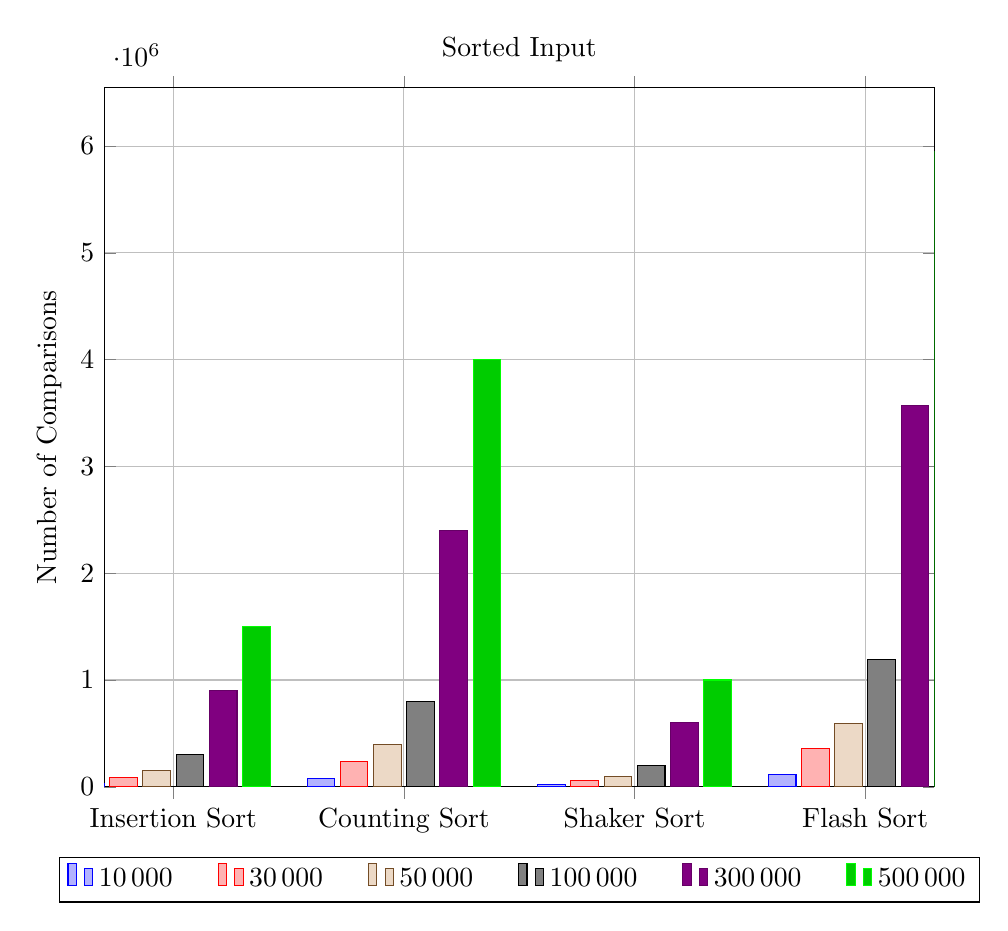
\begin{tikzpicture}
    \begin{axis}[
        width=\textwidth,
        title={Sorted Input},
        ybar,
        ymin=0,
        grid=major,
        legend style={
            at={(0.5,-0.1)}, anchor=north, legend columns=-1,
            /tikz/every even column/.append style={column sep=0.5cm}
        },
        ylabel={Number of Comparisons},
        symbolic x coords={Insertion Sort, Counting Sort, Shaker Sort, Flash Sort},
        xtick=data,
    ]
    \addplot coordinates {(Insertion Sort,29998) 
        (Counting Sort,80001) (Shaker Sort,20001) (Flash Sort,118993)};
    \addplot coordinates {(Insertion Sort,89998) 
        (Counting Sort,240001) (Shaker Sort,60001) (Flash Sort,356993)};
    \addplot coordinates {(Insertion Sort,149998) 
        (Counting Sort,400001) (Shaker Sort,100001) (Flash Sort,594993)};
    \addplot coordinates {(Insertion Sort,299998) 
        (Counting Sort,800001) (Shaker Sort,200001) (Flash Sort,1189993)};
    \addplot coordinates {(Insertion Sort,899998) 
        (Counting Sort,2400001) (Shaker Sort,600001) (Flash Sort,3569993)};
    \addplot coordinates {(Insertion Sort,1499998) 
        (Counting Sort,4000001) (Shaker Sort,1000001) (Flash Sort,5949993)};
    \legend{10\,000, 30\,000, 50\,000, 100\,000, 300\,000, 500\,000}
    \end{axis}
\end{tikzpicture}
\caption{Kết quả thực nghiệm với đầu vào có thứ tự đã được sắp xếp (Nhóm 3)}
\end{figure}

\begin{itemize}[label=$\circ$]
    \item Selection Sort, Shell Sort và Bubble Sort thực hiện một lượng 
    rất lớn số phép so sánh, đặc biệt là khi kích thước đầu vào lớn. Đó 
    là do các thuật toán này không có cách nào để “nhận ra” mảng đã được 
    sắp xếp xong nên liên tục thực hiện những phép so sánh vô nghĩa.
    \item Thuật toán Shaker Sort có số phép so sánh nhỏ nhất trong bảng 
    số liệu. Là một phiên bản cải tiến của Bubble Sort nên khi mảng đã 
    được sắp xếp sẵn, Shaker Sort chỉ cần duyệt qua mảng để xác nhận 
    rằng nó đã sắp xếp đúng, dẫn đến số phép so sánh rất thấp. Bên cạnh 
    đó, Insertion Sort cũng có số phép so sánh ít trong trường hợp mảng 
    đã được sắp xếp sẵn vì mỗi phần tử chỉ cần kiểm tra một lần với phần 
    tử liền trước để đảm bảo vị trí đúng mà không cần thực hiện thêm phép 
    so sánh nào khác.
\end{itemize}

$\bullet$ Với đầu vào có thứ tự được sắp xếp ngược \\

\begin{figure}[H]
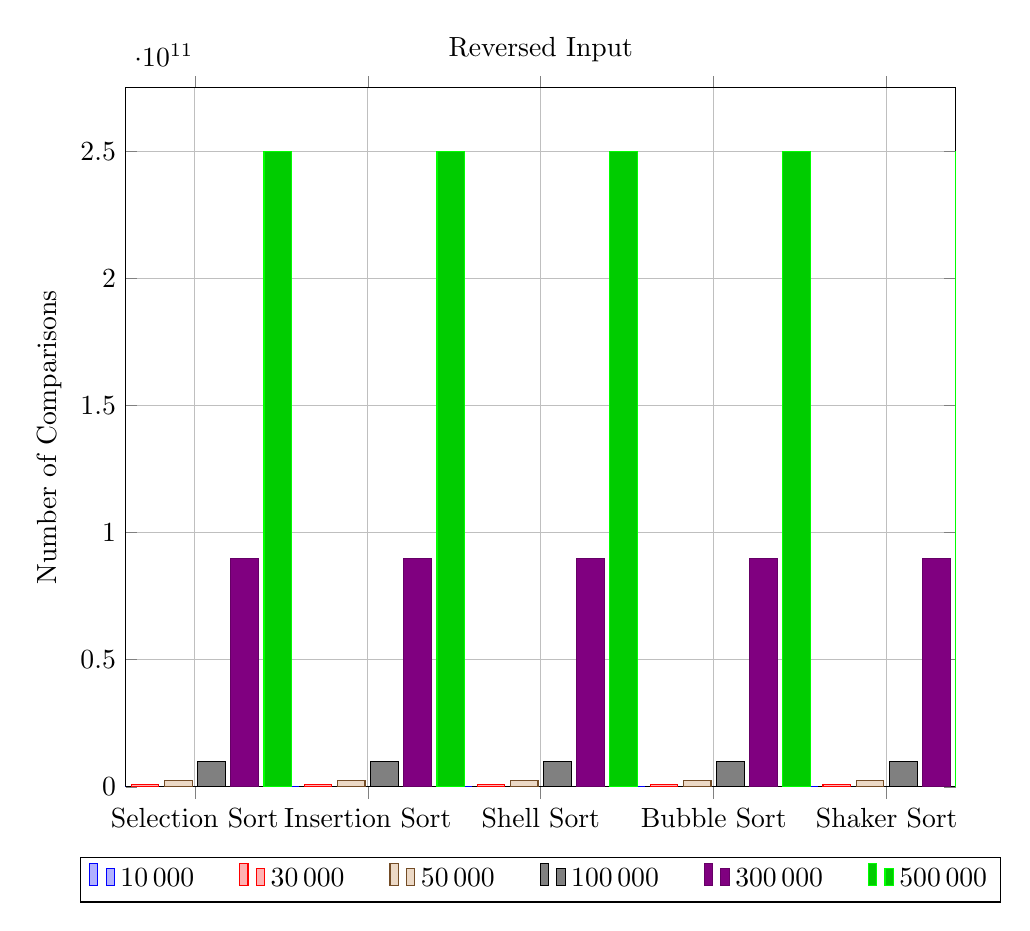
\begin{tikzpicture}
    \begin{axis}[
        width=\textwidth,
        title={Reversed Input},
        ybar,
        ymin=0,
        grid=major,
        legend style={
            at={(0.5,-0.1)}, anchor=north, legend columns=-1,
            /tikz/every even column/.append style={column sep=0.5cm}
        },
        ylabel={Number of Comparisons},
        symbolic x coords={Selection Sort, Insertion Sort, Shell Sort, Bubble Sort, Shaker Sort},
        xtick=data,
    ]
    \addplot coordinates {(Selection Sort,100009999) (Insertion Sort,100009999)
        (Shell Sort,100009999) (Bubble Sort,100009999) (Shaker Sort,100010001)};
    \addplot coordinates {(Selection Sort,900029999) (Insertion Sort,900029999)
        (Shell Sort,900029999) (Bubble Sort,900029999) (Shaker Sort,900030001)};
    \addplot coordinates {(Selection Sort,2500049999) (Insertion Sort,2500049999)
        (Shell Sort,2500049999) (Bubble Sort,2500049999) (Shaker Sort,2500050001)};
    \addplot coordinates {(Selection Sort,10000099999) (Insertion Sort,10000099999)
        (Shell Sort,10000099999) (Bubble Sort,10000099999) (Shaker Sort,10000100001)};
    \addplot coordinates {(Selection Sort,90000299999) (Insertion Sort,90000299999)
        (Shell Sort,90000299999) (Bubble Sort,90000299999) (Shaker Sort,90000300001)};
    \addplot coordinates {(Selection Sort,250000499999) (Insertion Sort,250000499999)
        (Shell Sort,250000499999) (Bubble Sort,250000499999) (Shaker Sort,250000500001)};
    \legend{10\,000, 30\,000, 50\,000, 100\,000, 300\,000, 500\,000}
    \end{axis}
\end{tikzpicture}
\caption{Kết quả thực nghiệm với đầu vào có thứ tự được sắp xếp ngược (Nhóm 1)}
\end{figure}

\begin{figure}[H]
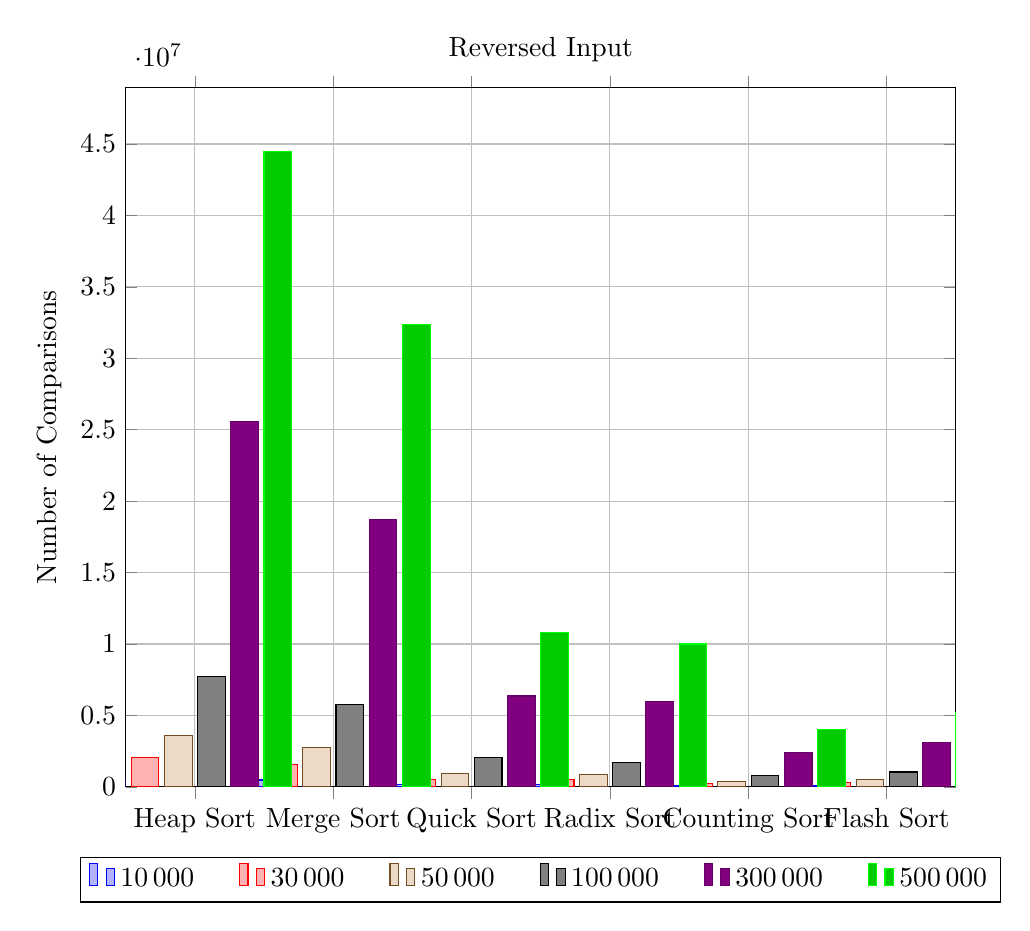
\begin{tikzpicture}
    \begin{axis}[
        width=\textwidth,
        title={Reversed Input},
        ybar,
        ymin=0,
        grid=major,
        legend style={
            at={(0.5,-0.1)}, anchor=north, legend columns=-1,
            /tikz/every even column/.append style={column sep=0.5cm}
        },
        ylabel={Number of Comparisons},
        symbolic x coords={Heap Sort, Merge Sort, Quick Sort, Radix Sort, Counting Sort, Flash Sort},
        xtick=data,
    ]
    \addplot coordinates {(Heap Sort,606771) (Merge Sort,476441) (Quick Sort,164975)
        (Radix Sort,140056) (Counting Sort,80001) (Flash Sort,103751)};
    \addplot coordinates {(Heap Sort,2063324) (Merge Sort,1573465) (Quick Sort,531939)
        (Radix Sort,510070) (Counting Sort,240001) (Flash Sort,311251)};
    \addplot coordinates {(Heap Sort,3612724) (Merge Sort,2733945) (Quick Sort,963861)
        (Radix Sort,850070) (Counting Sort,400001) (Flash Sort,518751)};
    \addplot coordinates {(Heap Sort,7718943) (Merge Sort,5767897) (Quick Sort,2027703)
        (Radix Sort,1700070) (Counting Sort,800001) (Flash Sort,1037501)};
    \addplot coordinates {(Heap Sort,25569379) (Merge Sort,18708313) (Quick Sort,6358249)
        (Radix Sort,6000084) (Counting Sort,2400001) (Flash Sort,3112501)};
    \addplot coordinates {(Heap Sort,44483348) (Merge Sort,32336409) (Quick Sort,10810747)
        (Radix Sort,10000084) (Counting Sort,4000001) (Flash Sort,5187501)};
    \legend{10\,000, 30\,000, 50\,000, 100\,000, 300\,000, 500\,000}
    \end{axis}
\end{tikzpicture}
\caption{Kết quả thực nghiệm với đầu vào có thứ tự được sắp xếp ngược (Nhóm 2)}
\end{figure}

\begin{itemize}[label=$\circ$]
    \item Selection Sort, Insertion Sort, Shell Sort, Bubble Sort và 
    Shaker Sort đều có số phép so sánh rất lớn trong trường hợp mảng được 
    sắp xếp ngược vì đây là trường hợp xấu nhất - mọi phần tử đều nằm sai 
    vị trí. Khi đó, các thuật toán này phải kiểm tra và điều chỉnh vị trí 
    của từng phần tử thông qua nhiều lần duyệt hoặc so sánh cặp.
    \item Counting Sort và Flash Sort có số phép so sánh thấp nhất trong 
    trường hợp này. Trong khi Counting Sort chỉ dựa trên việc đếm số lượng 
    phần tử trong các giá trị hoặc phạm vi thì Flash Sort sử dụng cách 
    phân chia mảng thành các nhóm dựa trên giá trị. Cả hai thuật toán này 
    đều hạn chế so sánh trực tiếp giữa các phần tử nên dù cho mảng có sắp 
    xếp ngược vẫn không ảnh hưởng quá nhiều.
\end{itemize}

$\blacktriangleright$ \textbf{Kết luận:}

[TO DO]
\pagebreak

% References
\cleardoublepage
\phantomsection
\addcontentsline{toc}{section}{Tài liệu tham khảo}
\bibliographystyle{unsrt}
\renewcommand{\refname}{Tài liệu tham khảo}
\bibliography{ref/ref}

\end{document}